% Options for packages loaded elsewhere
% Options for packages loaded elsewhere
\PassOptionsToPackage{unicode}{hyperref}
\PassOptionsToPackage{hyphens}{url}
\PassOptionsToPackage{dvipsnames,svgnames,x11names}{xcolor}
%
\documentclass[
  english,
  10pt,
  letterpaper,
  DIV=11,
  numbers=noendperiod]{scrartcl}
\usepackage{xcolor}
\usepackage[margin=1in]{geometry}
\usepackage{amsmath,amssymb}
\setcounter{secnumdepth}{5}
\usepackage{iftex}
\ifPDFTeX
  \usepackage[T1]{fontenc}
  \usepackage[utf8]{inputenc}
  \usepackage{textcomp} % provide euro and other symbols
\else % if luatex or xetex
  \usepackage{unicode-math} % this also loads fontspec
  \defaultfontfeatures{Scale=MatchLowercase}
  \defaultfontfeatures[\rmfamily]{Ligatures=TeX,Scale=1}
\fi
\usepackage{lmodern}
\ifPDFTeX\else
  % xetex/luatex font selection
\fi
% Use upquote if available, for straight quotes in verbatim environments
\IfFileExists{upquote.sty}{\usepackage{upquote}}{}
\IfFileExists{microtype.sty}{% use microtype if available
  \usepackage[]{microtype}
  \UseMicrotypeSet[protrusion]{basicmath} % disable protrusion for tt fonts
}{}
\makeatletter
\@ifundefined{KOMAClassName}{% if non-KOMA class
  \IfFileExists{parskip.sty}{%
    \usepackage{parskip}
  }{% else
    \setlength{\parindent}{0pt}
    \setlength{\parskip}{6pt plus 2pt minus 1pt}}
}{% if KOMA class
  \KOMAoptions{parskip=half}}
\makeatother
% Make \paragraph and \subparagraph free-standing
\makeatletter
\ifx\paragraph\undefined\else
  \let\oldparagraph\paragraph
  \renewcommand{\paragraph}{
    \@ifstar
      \xxxParagraphStar
      \xxxParagraphNoStar
  }
  \newcommand{\xxxParagraphStar}[1]{\oldparagraph*{#1}\mbox{}}
  \newcommand{\xxxParagraphNoStar}[1]{\oldparagraph{#1}\mbox{}}
\fi
\ifx\subparagraph\undefined\else
  \let\oldsubparagraph\subparagraph
  \renewcommand{\subparagraph}{
    \@ifstar
      \xxxSubParagraphStar
      \xxxSubParagraphNoStar
  }
  \newcommand{\xxxSubParagraphStar}[1]{\oldsubparagraph*{#1}\mbox{}}
  \newcommand{\xxxSubParagraphNoStar}[1]{\oldsubparagraph{#1}\mbox{}}
\fi
\makeatother

\usepackage{color}
\usepackage{fancyvrb}
\newcommand{\VerbBar}{|}
\newcommand{\VERB}{\Verb[commandchars=\\\{\}]}
\DefineVerbatimEnvironment{Highlighting}{Verbatim}{commandchars=\\\{\}}
% Add ',fontsize=\small' for more characters per line
\usepackage{framed}
\definecolor{shadecolor}{RGB}{241,243,245}
\newenvironment{Shaded}{\begin{snugshade}}{\end{snugshade}}
\newcommand{\AlertTok}[1]{\textcolor[rgb]{0.68,0.00,0.00}{#1}}
\newcommand{\AnnotationTok}[1]{\textcolor[rgb]{0.37,0.37,0.37}{#1}}
\newcommand{\AttributeTok}[1]{\textcolor[rgb]{0.40,0.45,0.13}{#1}}
\newcommand{\BaseNTok}[1]{\textcolor[rgb]{0.68,0.00,0.00}{#1}}
\newcommand{\BuiltInTok}[1]{\textcolor[rgb]{0.00,0.23,0.31}{#1}}
\newcommand{\CharTok}[1]{\textcolor[rgb]{0.13,0.47,0.30}{#1}}
\newcommand{\CommentTok}[1]{\textcolor[rgb]{0.37,0.37,0.37}{#1}}
\newcommand{\CommentVarTok}[1]{\textcolor[rgb]{0.37,0.37,0.37}{\textit{#1}}}
\newcommand{\ConstantTok}[1]{\textcolor[rgb]{0.56,0.35,0.01}{#1}}
\newcommand{\ControlFlowTok}[1]{\textcolor[rgb]{0.00,0.23,0.31}{\textbf{#1}}}
\newcommand{\DataTypeTok}[1]{\textcolor[rgb]{0.68,0.00,0.00}{#1}}
\newcommand{\DecValTok}[1]{\textcolor[rgb]{0.68,0.00,0.00}{#1}}
\newcommand{\DocumentationTok}[1]{\textcolor[rgb]{0.37,0.37,0.37}{\textit{#1}}}
\newcommand{\ErrorTok}[1]{\textcolor[rgb]{0.68,0.00,0.00}{#1}}
\newcommand{\ExtensionTok}[1]{\textcolor[rgb]{0.00,0.23,0.31}{#1}}
\newcommand{\FloatTok}[1]{\textcolor[rgb]{0.68,0.00,0.00}{#1}}
\newcommand{\FunctionTok}[1]{\textcolor[rgb]{0.28,0.35,0.67}{#1}}
\newcommand{\ImportTok}[1]{\textcolor[rgb]{0.00,0.46,0.62}{#1}}
\newcommand{\InformationTok}[1]{\textcolor[rgb]{0.37,0.37,0.37}{#1}}
\newcommand{\KeywordTok}[1]{\textcolor[rgb]{0.00,0.23,0.31}{\textbf{#1}}}
\newcommand{\NormalTok}[1]{\textcolor[rgb]{0.00,0.23,0.31}{#1}}
\newcommand{\OperatorTok}[1]{\textcolor[rgb]{0.37,0.37,0.37}{#1}}
\newcommand{\OtherTok}[1]{\textcolor[rgb]{0.00,0.23,0.31}{#1}}
\newcommand{\PreprocessorTok}[1]{\textcolor[rgb]{0.68,0.00,0.00}{#1}}
\newcommand{\RegionMarkerTok}[1]{\textcolor[rgb]{0.00,0.23,0.31}{#1}}
\newcommand{\SpecialCharTok}[1]{\textcolor[rgb]{0.37,0.37,0.37}{#1}}
\newcommand{\SpecialStringTok}[1]{\textcolor[rgb]{0.13,0.47,0.30}{#1}}
\newcommand{\StringTok}[1]{\textcolor[rgb]{0.13,0.47,0.30}{#1}}
\newcommand{\VariableTok}[1]{\textcolor[rgb]{0.07,0.07,0.07}{#1}}
\newcommand{\VerbatimStringTok}[1]{\textcolor[rgb]{0.13,0.47,0.30}{#1}}
\newcommand{\WarningTok}[1]{\textcolor[rgb]{0.37,0.37,0.37}{\textit{#1}}}

\usepackage{longtable,booktabs,array}
\newcounter{none} % for unnumbered tables
\usepackage{calc} % for calculating minipage widths
% Correct order of tables after \paragraph or \subparagraph
\usepackage{etoolbox}
\makeatletter
\patchcmd\longtable{\par}{\if@noskipsec\mbox{}\fi\par}{}{}
\makeatother
% Allow footnotes in longtable head/foot
\IfFileExists{footnotehyper.sty}{\usepackage{footnotehyper}}{\usepackage{footnote}}
\makesavenoteenv{longtable}
\usepackage{graphicx}
\makeatletter
\newsavebox\pandoc@box
\newcommand*\pandocbounded[1]{% scales image to fit in text height/width
  \sbox\pandoc@box{#1}%
  \Gscale@div\@tempa{\textheight}{\dimexpr\ht\pandoc@box+\dp\pandoc@box\relax}%
  \Gscale@div\@tempb{\linewidth}{\wd\pandoc@box}%
  \ifdim\@tempb\p@<\@tempa\p@\let\@tempa\@tempb\fi% select the smaller of both
  \ifdim\@tempa\p@<\p@\scalebox{\@tempa}{\usebox\pandoc@box}%
  \else\usebox{\pandoc@box}%
  \fi%
}
% Set default figure placement to htbp
\def\fps@figure{htbp}
\makeatother


% definitions for citeproc citations
\NewDocumentCommand\citeproctext{}{}
\NewDocumentCommand\citeproc{mm}{%
  \begingroup\def\citeproctext{#2}\cite{#1}\endgroup}
\makeatletter
 % allow citations to break across lines
 \let\@cite@ofmt\@firstofone
 % avoid brackets around text for \cite:
 \def\@biblabel#1{}
 \def\@cite#1#2{{#1\if@tempswa , #2\fi}}
\makeatother
\newlength{\cslhangindent}
\setlength{\cslhangindent}{1.5em}
\newlength{\csllabelwidth}
\setlength{\csllabelwidth}{3em}
\newenvironment{CSLReferences}[2] % #1 hanging-indent, #2 entry-spacing
 {\begin{list}{}{%
  \setlength{\itemindent}{0pt}
  \setlength{\leftmargin}{0pt}
  \setlength{\parsep}{0pt}
  % turn on hanging indent if param 1 is 1
  \ifodd #1
   \setlength{\leftmargin}{\cslhangindent}
   \setlength{\itemindent}{-1\cslhangindent}
  \fi
  % set entry spacing
  \setlength{\itemsep}{#2\baselineskip}}}
 {\end{list}}
\usepackage{calc}
\newcommand{\CSLBlock}[1]{\hfill\break\parbox[t]{\linewidth}{\strut\ignorespaces#1\strut}}
\newcommand{\CSLLeftMargin}[1]{\parbox[t]{\csllabelwidth}{\strut#1\strut}}
\newcommand{\CSLRightInline}[1]{\parbox[t]{\linewidth - \csllabelwidth}{\strut#1\strut}}
\newcommand{\CSLIndent}[1]{\hspace{\cslhangindent}#1}

\ifLuaTeX
\usepackage[bidi=basic,shorthands=off]{babel}
\else
\usepackage[bidi=default,shorthands=off]{babel}
\fi
\ifLuaTeX
  \usepackage{selnolig} % disable illegal ligatures
\fi


\setlength{\emergencystretch}{3em} % prevent overfull lines

\providecommand{\tightlist}{%
  \setlength{\itemsep}{0pt}\setlength{\parskip}{0pt}}



 


\KOMAoption{captions}{tableheading}
\makeatletter
\@ifpackageloaded{caption}{}{\usepackage{caption}}
\AtBeginDocument{%
\ifdefined\contentsname
  \renewcommand*\contentsname{Table of contents}
\else
  \newcommand\contentsname{Table of contents}
\fi
\ifdefined\listfigurename
  \renewcommand*\listfigurename{List of Figures}
\else
  \newcommand\listfigurename{List of Figures}
\fi
\ifdefined\listtablename
  \renewcommand*\listtablename{List of Tables}
\else
  \newcommand\listtablename{List of Tables}
\fi
\ifdefined\figurename
  \renewcommand*\figurename{Figure}
\else
  \newcommand\figurename{Figure}
\fi
\ifdefined\tablename
  \renewcommand*\tablename{Table}
\else
  \newcommand\tablename{Table}
\fi
}
\@ifpackageloaded{float}{}{\usepackage{float}}
\floatstyle{ruled}
\@ifundefined{c@chapter}{\newfloat{codelisting}{h}{lop}}{\newfloat{codelisting}{h}{lop}[chapter]}
\floatname{codelisting}{Listing}
\newcommand*\listoflistings{\listof{codelisting}{List of Listings}}
\usepackage{amsthm}
\theoremstyle{plain}
\newtheorem{theorem}{Theorem}[section]
\theoremstyle{remark}
\AtBeginDocument{\renewcommand*{\proofname}{Proof}}
\newtheorem*{remark}{Remark}
\newtheorem*{solution}{Solution}
\newtheorem{refremark}{Remark}[section]
\newtheorem{refsolution}{Solution}[section]
\makeatother
\makeatletter
\makeatother
\makeatletter
\@ifpackageloaded{caption}{}{\usepackage{caption}}
\@ifpackageloaded{subcaption}{}{\usepackage{subcaption}}
\makeatother
\usepackage{bookmark}
\IfFileExists{xurl.sty}{\usepackage{xurl}}{} % add URL line breaks if available
\urlstyle{same}
\hypersetup{
  pdftitle={A Faithful One-Driver Complex Embedding of Arithmetic Brownian Motion},
  pdfauthor={Complex--Itô Random-Walk Research Project},
  pdflang={en},
  pdfkeywords={Itô calculus, complex stochastic process, arithmetic
Brownian motion, logarithmic spiral, covariance rank, quadratic
variation, local time, Tanaka formula},
  colorlinks=true,
  linkcolor={blue},
  filecolor={Maroon},
  citecolor={Blue},
  urlcolor={Blue},
  pdfcreator={LaTeX via pandoc}}


\title{A Faithful One-Driver Complex Embedding of Arithmetic Brownian
Motion}
\usepackage{etoolbox}
\makeatletter
\providecommand{\subtitle}[1]{% add subtitle to \maketitle
  \apptocmd{\@title}{\par {\large #1 \par}}{}{}
}
\makeatother
\subtitle{Itô dynamics, covariance rank, and zero crossings}
\author{Complex--Itô Random-Walk Research Project}
\date{July 23, 2026}
\begin{document}
\maketitle
\begin{abstract}
We study how a scalar arithmetic Brownian motion can be represented by a
complex exponential whose radius and angle are both stochastic without
introducing a second Brownian driver. For \(dX_t=\mu\,dt+\sigma\,dW_t\),
\(c=\alpha+i\beta\), and \(Z_t=Z_0\exp(c(X_t-X_0))\), the radius
recovers the scalar state whenever \(\alpha\ne0\), while the unwrapped
angle and log-radius lie on a deterministic line. We derive the induced
complex Itô equation, exact finite-step multiplicative walk,
distributions, moments, and both the bilinear and Hermitian complex
quadratic variations. A general rank theorem shows that every smooth
complex image of a scalar diffusion has instantaneous Cartesian
covariance of rank at most one. This distinguishes the embedding from
planar Brownian motion, whose local covariance has rank two. We also
explain why the literal polar representation of a signed scalar process
is only local before a zero and why Tanaka local time is required
globally. Symbolic checks, exact-path identities, Monte Carlo estimates,
shared-path strong-convergence experiments, and local-time
approximations are preserved in an executable discovery notebook. The
construction is an information-preserving geometric representation of
one-dimensional noise, not a relabelling of planar Brownian motion.
\end{abstract}

\renewcommand*\contentsname{Table of contents}
{
\setcounter{tocdepth}{2}
\tableofcontents
}

\section{Introduction}\label{sec-introduction}

The symbolic rule

\[
(dW_t)^2=dt
\]

and the algebraic identity \(i^2=-1\) look tantalizingly similar. They
are not the same kind of statement. The first abbreviates a
quadratic-variation limit; the second is an exact identity in the
complex numbers. Nevertheless, complex multiplication is valuable for
organizing stochastic scale and rotation. The question is how to use
that geometry without changing the underlying stochastic model.

Let

\begin{equation}\protect\phantomsection\label{eq-scalar-sde}{
dX_t=\mu\,dt+\sigma\,dW_t,\qquad X_0\in\mathbb R,
}\end{equation}

where \(W\) is one standard real Brownian motion. We seek a complex
process whose radius and angle both fluctuate, which contains exactly
the information in \(X\), and which is still driven by this one \(W\).
The central construction is

\begin{equation}\protect\phantomsection\label{eq-central-map}{
\boxed{
Z_t=Z_0\exp\!\left(c(X_t-X_0)\right),\qquad
c=\alpha+i\beta,\quad \alpha\ne0.
}
}\end{equation}

Its polar coordinates are

\begin{equation}\protect\phantomsection\label{eq-polar-coordinates}{
\log R_t=\log R_0+\alpha(X_t-X_0),\qquad
\Theta_t=\Theta_0+\beta(X_t-X_0).
}\end{equation}

Both coordinates are stochastic if \(\alpha\beta\ne0\), but they share
one Brownian direction. The resulting path lies on a logarithmic spiral
and has rank-one instantaneous covariance. That rank is the mathematical
distinction between a faithful complex embedding of scalar Brownian
motion and a genuine two-driver Brownian motion in the plane.

\begin{figure}[H]

\centering{

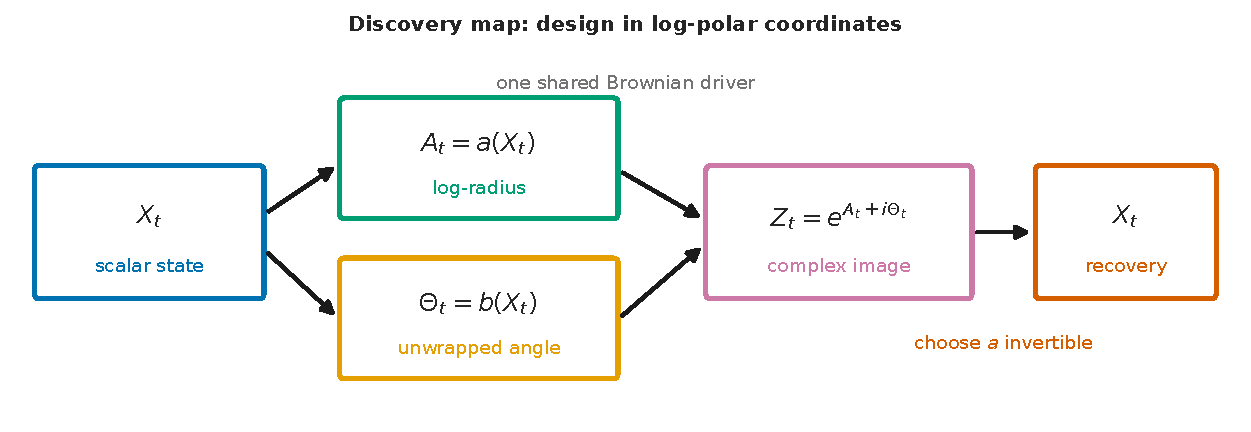
\includegraphics[width=1\linewidth,height=\textheight,keepaspectratio,alt={A flow diagram maps the scalar process X into log-radius A and angle Theta, combines them as the complex exponential Z, and recovers X from an invertible radial map.}]{figures/vector/f01_discovery_map.pdf}

}

\caption{\label{fig-discovery-map}Starting from a scalar state, design
log-radius and unwrapped angle as functions of that state, reconstruct a
complex variable, and recover the state through an invertible radius
map.}

\end{figure}%

Figure~\ref{fig-discovery-map} summarizes the constructive strategy. The
contribution is a rigorous synthesis and visual account of standard Itô
tools applied to this specific design problem. We do \textbf{not} claim
that the exponential map, the logarithmic spiral, or the outer-product
rank calculation is a new theorem.

The main results are:

\begin{enumerate}
\def\labelenumi{\arabic{enumi}.}
\tightlist
\item
  an injective one-driver complex embedding with stochastic radius and
  angle;
\item
  two matching derivations of its complex Itô equation;
\item
  exact state recovery and an exact finite-step multiplicative random
  walk;
\item
  a general rank-one obstruction for smooth complex images of scalar
  diffusions;
\item
  explicit complex brackets, distributions, and moments; and
\item
  a localized and global treatment of scalar zero crossings.
\end{enumerate}

\section{Literature and positioning}\label{sec-literature}

The multidimensional Itô formula and the covariance factorization
\(\Sigma\Sigma^\mathsf T\) are standard. We use them componentwise for
complex maps, treating \(\mathbb C\) as \(\mathbb R^2\); accessible
derivations appear in Goodman's stochastic-calculus notes and the broad
survey by Pitman and Yor (Goodman 2007; Pitman and Yor 2018).

The distinction between stochastic exponentials and stochastic
logarithms is important near zeros. Larsson and Ruf formulate these
transforms on stochastic intervals and make explicit why continuous
hitting of zero matters (Larsson and Ruf 2019). Brownian local time,
occupation density, and Tanaka's formula are standard tools for the
nonsmooth absolute-value map (Mörters and Peres 2010; Biskup 2025).

Planar Brownian motion supplies a necessary control, not an alternative
description of the scalar model. Its radial Bessel behavior, nonhitting
of a fixed point when started elsewhere, and winding process belong to a
genuinely two-dimensional theory (Pitman and Yor 2018, 1986). The
numerical strong-convergence experiment follows the shared-Brownian-path
methodology used in expositions of Euler--Maruyama (Higham 2001).

The particular synthesis developed below---designing a recoverable
log-polar embedding, stating its noise-rank obstruction, and relating it
to exact complex random-walk steps---is derived directly from these
standard tools. The paper is therefore best read as an expository
computational mathematics note.

\section{Preliminaries and notation}\label{sec-preliminaries}

We identify \(z=x+iy\in\mathbb C\) with \((x,y)\in\mathbb R^2\). For a
complex continuous semimartingale \(Z=U+iV\), define

\begin{equation}\protect\phantomsection\label{eq-bilinear-bracket}{
[Z,Z]=[U,U]-[V,V]+2i[U,V]
}\end{equation}

and

\begin{equation}\protect\phantomsection\label{eq-hermitian-bracket}{
[Z,\overline Z]=[U,U]+[V,V].
}\end{equation}

The first is complex bilinear and can exhibit phase cancellation. The
second is Hermitian, real, and nonnegative.

The angle \(\Theta\) in this paper is an \emph{unwrapped} continuous
lift, not merely an element of \(\mathbb R/(2\pi\mathbb Z)\). This
distinction matters when discussing recovery from phase.

\begin{longtable}[]{@{}ll@{}}
\caption{Core notation.}\label{tbl-notation}\tabularnewline
\toprule\noalign{}
Symbol & Meaning \\
\midrule\noalign{}
\endfirsthead
\toprule\noalign{}
Symbol & Meaning \\
\midrule\noalign{}
\endhead
\bottomrule\noalign{}
\endlastfoot
\(X_t\) & scalar arithmetic Brownian motion \\
\(W_t\) & one standard real Brownian driver \\
\(\mu,\sigma\) & scalar drift and volatility, with \(\sigma>0\) \\
\(Z_t\) & complex embedding \\
\(R_t=\lvert Z_t\rvert\) & stochastic radius \\
\(\Theta_t\) & unwrapped stochastic angle \\
\(A_t=\log R_t\) & log-radius \\
\(c=\alpha+i\beta\) & complex embedding parameter \\
\([Y_1,Y_2]_t\) & quadratic covariation \\
\(\tau_0\) & first hitting time of zero by a scalar process \\
\(L_t^0(X)\) & symmetric local time of \(X\) at zero \\
\end{longtable}

Three levels of equality will be kept separate:

\begin{itemize}
\tightlist
\item
  a \textbf{pathwise identity}, such as Eq.~\ref{eq-central-map};
\item
  an \textbf{Itô differential identity}, determined by finite variation
  and quadratic covariation; and
\item
  a \textbf{mnemonic}, such as \((dW)^2=dt\), which must not be read as
  an ordinary finite-increment algebraic equation.
\end{itemize}

\section{Problem formulation}\label{sec-problem}

The word \emph{representation} can mean several different things.

\begin{longtable}[]{@{}
  >{\raggedright\arraybackslash}p{(\linewidth - 4\tabcolsep) * \real{0.3333}}
  >{\raggedright\arraybackslash}p{(\linewidth - 4\tabcolsep) * \real{0.3333}}
  >{\raggedright\arraybackslash}p{(\linewidth - 4\tabcolsep) * \real{0.3333}}@{}}
\caption{Four meanings of
representation.}\label{tbl-representation}\tabularnewline
\toprule\noalign{}
\begin{minipage}[b]{\linewidth}\raggedright
Meaning
\end{minipage} & \begin{minipage}[b]{\linewidth}\raggedright
Requirement
\end{minipage} & \begin{minipage}[b]{\linewidth}\raggedright
What it preserves
\end{minipage} \\
\midrule\noalign{}
\endfirsthead
\toprule\noalign{}
\begin{minipage}[b]{\linewidth}\raggedright
Meaning
\end{minipage} & \begin{minipage}[b]{\linewidth}\raggedright
Requirement
\end{minipage} & \begin{minipage}[b]{\linewidth}\raggedright
What it preserves
\end{minipage} \\
\midrule\noalign{}
\endhead
\bottomrule\noalign{}
\endlastfoot
Deterministic image & \(Z_t=F(X_t)\) & a chosen geometric view \\
State-injective embedding & \(F\) is injective & pointwise scalar
state \\
Pathwise recovery & the lifted \(Z\)-path determines \(X\) & path
information \\
Planar-model equality & the local law and covariance match a target in
\(\mathbb R^2\) & full planar stochastic model \\
\end{longtable}

\begin{figure}[H]

\centering{

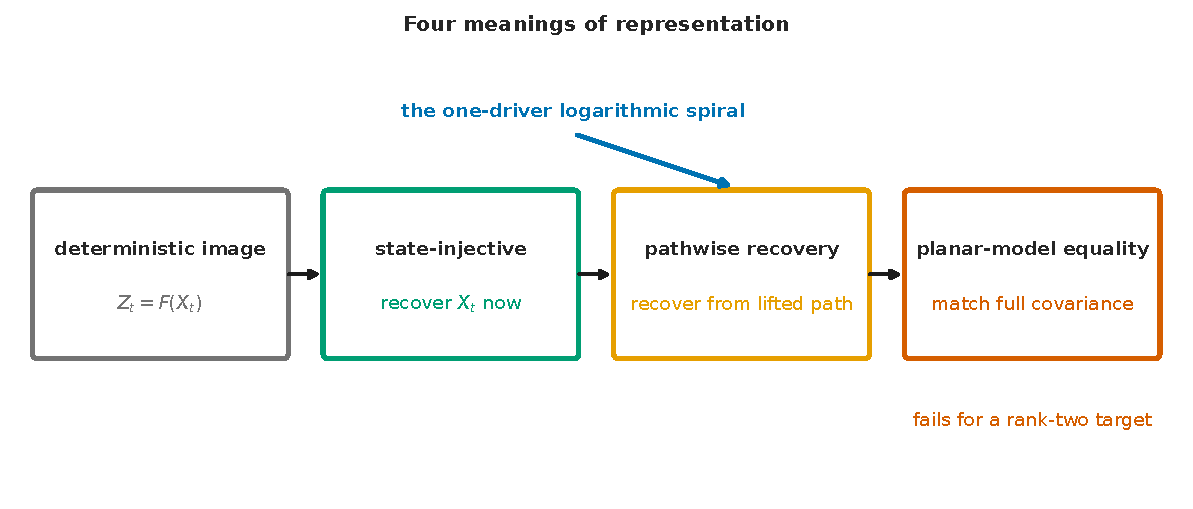
\includegraphics[width=1\linewidth,height=\textheight,keepaspectratio,alt={Four boxes progress from deterministic image to state injection, pathwise recovery, and planar model equality. An arrow marks the one-driver logarithmic spiral through the first three and states that it fails the rank-two target.}]{figures/vector/f16_representation_taxonomy.pdf}

}

\caption{\label{fig-representation-taxonomy}The logarithmic spiral
satisfies deterministic image, state-injective embedding, and pathwise
recovery, but it cannot equal a full-rank planar Brownian model.}

\end{figure}%

The desired object must satisfy the first three notions while retaining
one Brownian driver. The fourth is neither required nor possible for a
rank-two target. Figure~\ref{fig-representation-taxonomy} makes this
hierarchy explicit.

Write general log-polar coordinates as

\begin{equation}\protect\phantomsection\label{eq-general-log-polar}{
A_t=a(X_t),\qquad \Theta_t=b(X_t),\qquad
Z_t=e^{A_t+i\Theta_t}.
}\end{equation}

For \(C^2\) functions \(a,b\), scalar Itô calculus already guarantees
that the two coordinates share one driver:

\begin{equation}\protect\phantomsection\label{eq-general-polar-ito}{
\begin{aligned}
dA_t
&=\left(\mu a'(X_t)+\tfrac12\sigma^2a''(X_t)\right)dt
  +\sigma a'(X_t)dW_t,\\
d\Theta_t
&=\left(\mu b'(X_t)+\tfrac12\sigma^2b''(X_t)\right)dt
  +\sigma b'(X_t)dW_t.
\end{aligned}
}\end{equation}

Thus the design problem becomes deterministic: choose \(a\) invertible
for state recovery and choose both derivatives nonzero for stochastic
radius and angle.

\section{The logarithmic-spiral construction}\label{sec-construction}

The simplest globally smooth choice is affine:

\begin{equation}\protect\phantomsection\label{eq-affine-log-polar}{
a(x)=\log R_0+\alpha(x-X_0),\qquad
b(x)=\Theta_0+\beta(x-X_0).
}\end{equation}

Substitution in Eq.~\ref{eq-general-log-polar} gives
Eq.~\ref{eq-central-map}.

\begin{theorem}[Faithful one-driver
embedding]\protect\hypertarget{thm-embedding}{}\label{thm-embedding}

Let \(X\) satisfy Eq.~\ref{eq-scalar-sde}, let \(Z_0\ne0\), and let
\(c=\alpha+i\beta\) with \(\alpha\ne0\). Then the process in
Eq.~\ref{eq-central-map} is nonvanishing and state-injective.
Specifically,

\begin{equation}\protect\phantomsection\label{eq-inverse-radius}{
\boxed{
X_t=X_0+\frac1\alpha\log\frac{|Z_t|}{|Z_0|}.
}
}\end{equation}

Consequently, after completion in the usual way,
\(\sigma(Z_s:0\le s\le t)=\sigma(X_s:0\le s\le t)\) for each \(t\).

\end{theorem}

The proof is immediate from \(|Z_t|=R_0e^{\alpha(X_t-X_0)}\). The
formula also shows why the lifted angle is not needed for recovery when
\(\alpha\ne0\).

Eliminating \(X_t-X_0\) from Eq.~\ref{eq-polar-coordinates} gives

\begin{equation}\protect\phantomsection\label{eq-spiral-relation}{
\boxed{
\Theta_t-\Theta_0
=\frac{\beta}{\alpha}\log\frac{R_t}{R_0}.
}
}\end{equation}

Thus the two visible polar coordinates are exactly coupled.

\begin{figure}[H]

\centering{

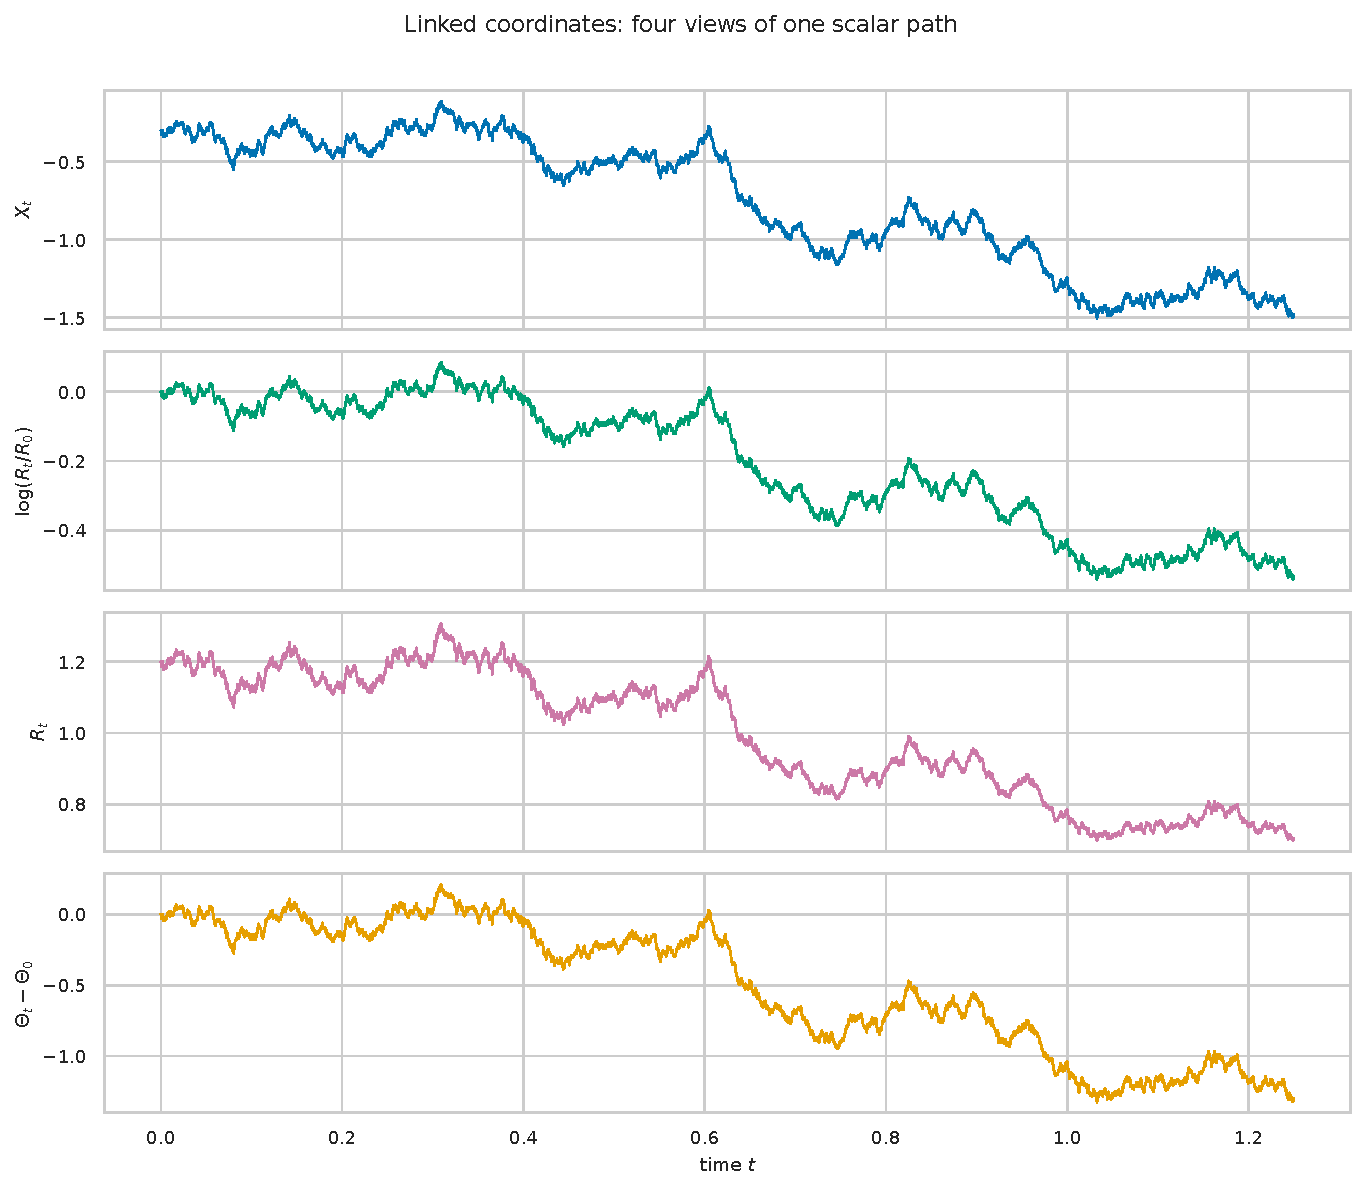
\includegraphics[width=0.92\linewidth,height=\textheight,keepaspectratio,alt={Four stacked time-series panels show X, log R over R0, R, and unwrapped angle. All features occur at the same times, illustrating the shared scalar driver.}]{figures/vector/f02_linked_path.pdf}

}

\caption{\label{fig-linked-path}The scalar path, log-radius, radius, and
unwrapped angle share every reversal because they are deterministic
functions of one state.}

\end{figure}%

\begin{figure}[H]

\centering{

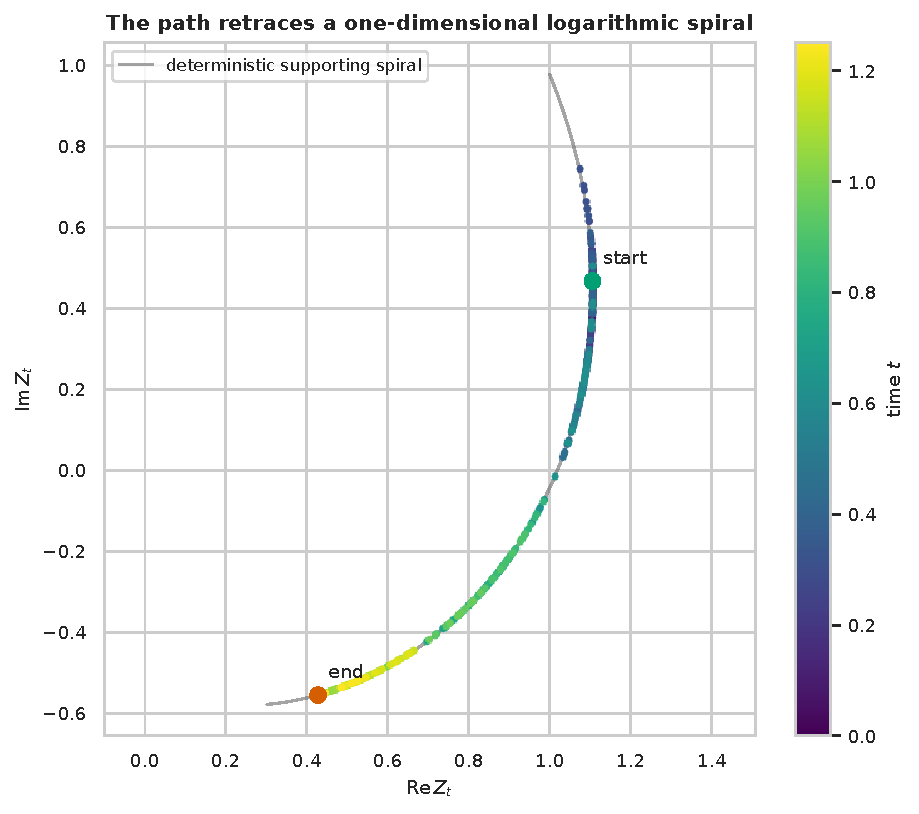
\includegraphics[width=0.72\linewidth,height=\textheight,keepaspectratio,alt={A gray logarithmic spiral supports colored sample points ordered by time. The process moves back and forth along the same curve rather than diffusing across planar area.}]{figures/vector/f03_complex_spiral.pdf}

}

\caption{\label{fig-complex-spiral}A time-colored sample path lies on
and repeatedly retraces one deterministic logarithmic spiral.}

\end{figure}%

The parameter cases are:

\begin{longtable}[]{@{}
  >{\raggedright\arraybackslash}p{(\linewidth - 4\tabcolsep) * \real{0.3333}}
  >{\raggedright\arraybackslash}p{(\linewidth - 4\tabcolsep) * \real{0.3333}}
  >{\raggedright\arraybackslash}p{(\linewidth - 4\tabcolsep) * \real{0.3333}}@{}}
\caption{Parameter
classification.}\label{tbl-parameter-cases}\tabularnewline
\toprule\noalign{}
\begin{minipage}[b]{\linewidth}\raggedright
Parameters
\end{minipage} & \begin{minipage}[b]{\linewidth}\raggedright
Geometry
\end{minipage} & \begin{minipage}[b]{\linewidth}\raggedright
Stochastic information
\end{minipage} \\
\midrule\noalign{}
\endfirsthead
\toprule\noalign{}
\begin{minipage}[b]{\linewidth}\raggedright
Parameters
\end{minipage} & \begin{minipage}[b]{\linewidth}\raggedright
Geometry
\end{minipage} & \begin{minipage}[b]{\linewidth}\raggedright
Stochastic information
\end{minipage} \\
\midrule\noalign{}
\endhead
\bottomrule\noalign{}
\endlastfoot
\(\alpha=0,\ \beta\ne0\) & circle & radius loses the state; lifted phase
can retain it \\
\(\alpha\ne0,\ \beta=0\) & ray & radius alone is injective \\
\(\alpha\beta\ne0\) & logarithmic spiral & radius and angle fluctuate,
rank one \\
\(\alpha=\beta=0\) & one point & all state information is lost \\
\end{longtable}

\begin{figure}[H]

\centering{

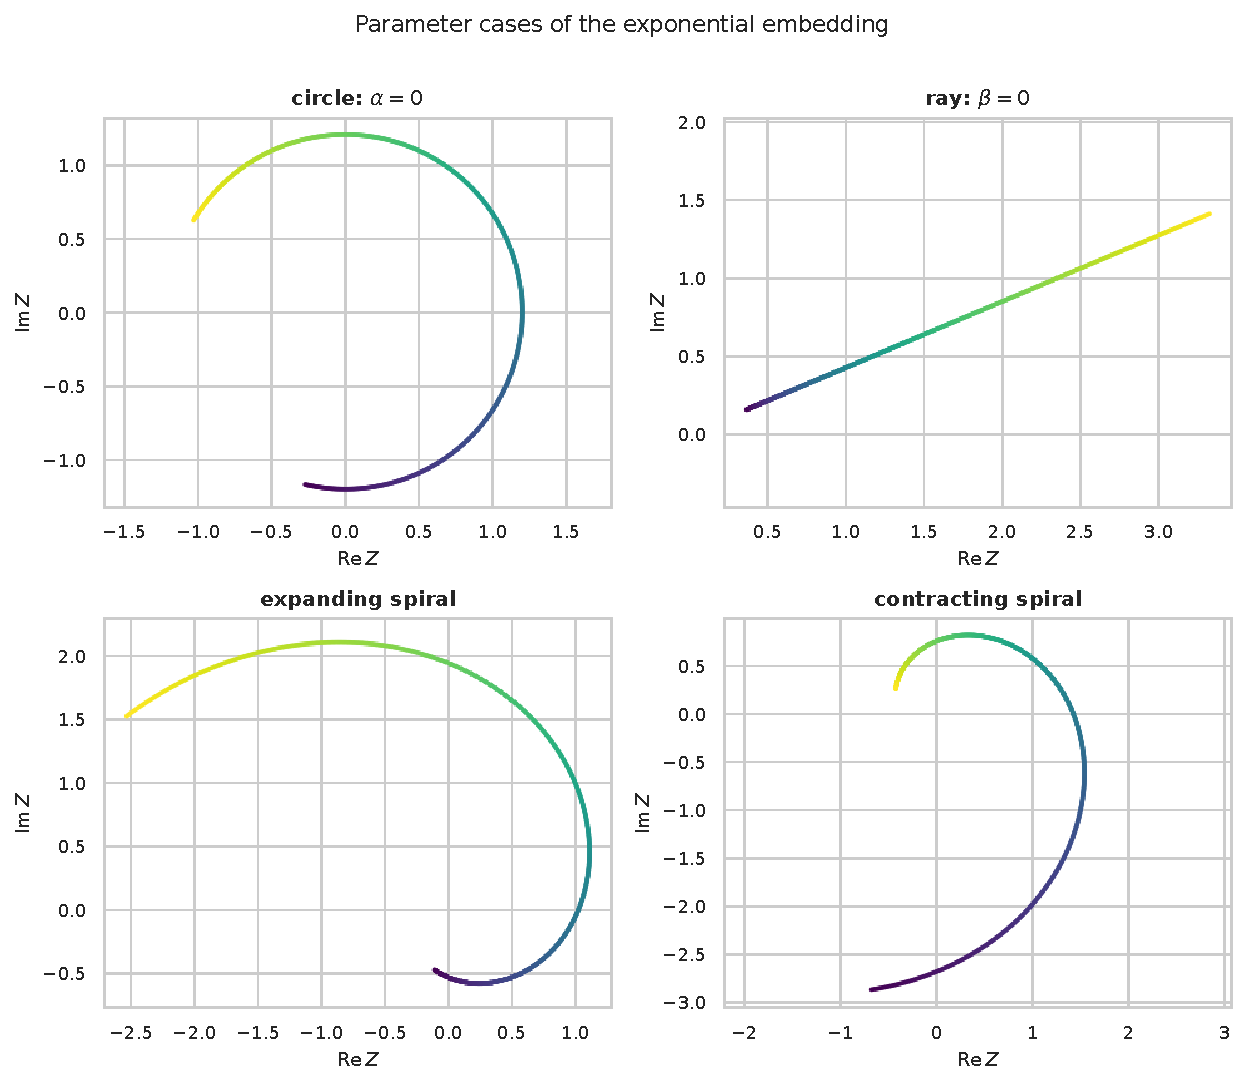
\includegraphics[width=0.82\linewidth,height=\textheight,keepaspectratio,alt={A four-panel gallery shows the geometric support for pure rotation, pure radial scaling, expanding spiral, and contracting spiral parameter choices.}]{figures/vector/f05_parameter_gallery.pdf}

}

\caption{\label{fig-parameter-gallery}Changing alpha and beta produces a
circle, a ray, an expanding spiral, or a contracting spiral.}

\end{figure}%

\section{Itô dynamics and the exact random walk}\label{sec-ito}

Let \(F(x)=Z_0e^{c(x-X_0)}\). Since \(F'=cF\) and \(F''=c^2F\), scalar
Itô calculus gives

\begin{equation}\protect\phantomsection\label{eq-complex-sde}{
\boxed{
\frac{dZ_t}{Z_t}
=\left(c\mu+\frac12c^2\sigma^2\right)dt
+c\sigma\,dW_t.
}
}\end{equation}

Equivalently,

\begin{equation}\protect\phantomsection\label{eq-linear-complex-sde}{
dZ_t=\lambda Z_t\,dt+\nu Z_t\,dW_t,\qquad
\lambda=c\mu+\tfrac12c^2\sigma^2,\quad \nu=c\sigma.
}\end{equation}

The differential \(dZ_t/Z_t\) in Eq.~\ref{eq-complex-sde} is the
stochastic logarithm differential of \(Z\) (Larsson and Ruf 2019).

There is an independent polar derivation. From
Eq.~\ref{eq-polar-coordinates},

\begin{equation}\protect\phantomsection\label{eq-linear-polar-sde}{
dA_t=\alpha\mu\,dt+\alpha\sigma\,dW_t,\qquad
d\Theta_t=\beta\mu\,dt+\beta\sigma\,dW_t.
}\end{equation}

For \(Z=e^{A+i\Theta}\), two-dimensional Itô calculus yields

\begin{equation}\protect\phantomsection\label{eq-polar-reconstruction}{
\frac{dZ}{Z}
=dA+i\,d\Theta
+\frac12\left(d[A,A]-d[\Theta,\Theta]\right)
+i\,d[A,\Theta].
}\end{equation}

Using

\begin{equation}\protect\phantomsection\label{eq-polar-brackets}{
d[A,A]=\alpha^2\sigma^2dt,\quad
d[\Theta,\Theta]=\beta^2\sigma^2dt,\quad
d[A,\Theta]=\alpha\beta\sigma^2dt
}\end{equation}

reduces Eq.~\ref{eq-polar-reconstruction} exactly to
Eq.~\ref{eq-complex-sde}. The mixed covariation is essential; omitting
it loses the imaginary Itô correction.

Because Eq.~\ref{eq-central-map} is pathwise, a grid increment has the
exact update

\begin{equation}\protect\phantomsection\label{eq-exact-step}{
\boxed{
Z_{n+1}=Z_n\exp\!\left(c\,\Delta X_n\right),\qquad
\Delta X_n=\mu\,\Delta t+\sigma\,\Delta W_n.
}
}\end{equation}

\begin{figure}[H]

\centering{

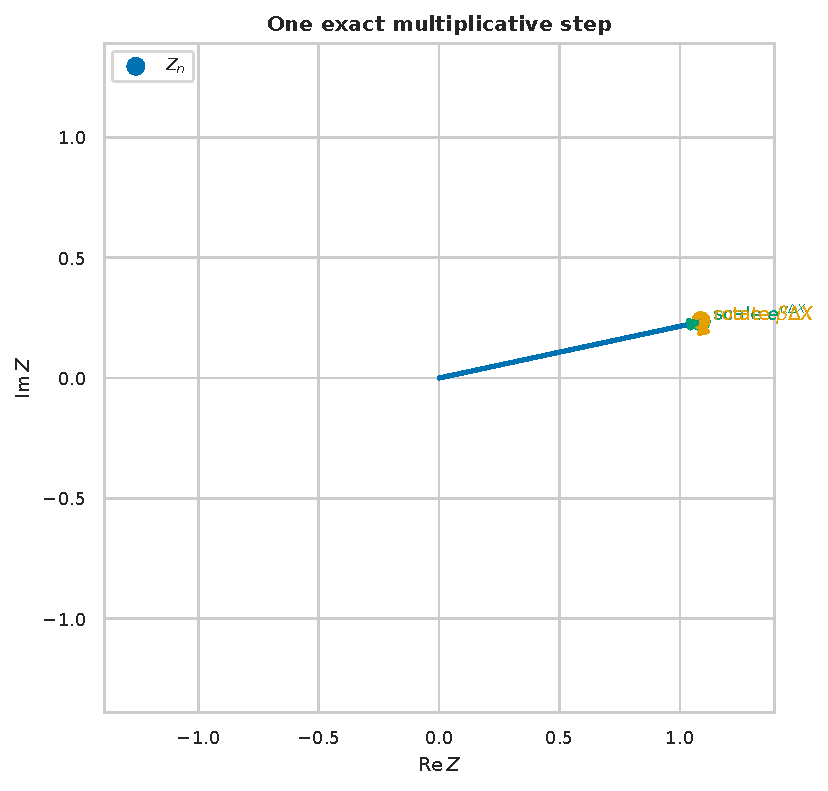
\includegraphics[width=0.7\linewidth,height=\textheight,keepaspectratio,alt={A complex-plane vector Z n is radially scaled by exp alpha Delta X and rotated by beta Delta X to reach Z n plus 1.}]{figures/vector/f09_exact_multiplicative_step.pdf}

}

\caption{\label{fig-exact-step}One scalar increment first appears as
radial scaling and then as angular rotation; together they equal the
exact complex factor.}

\end{figure}%

Eq.~\ref{eq-exact-step} is not Euler--Maruyama. It is exact at every
grid point because the exponential factors telescope.

The diffusion coefficient in Eq.~\ref{eq-complex-sde} is
\(c\sigma Z_t\), a single complex vector. It determines one
instantaneous direction in \(\mathbb R^2\), even though the direction
rotates with the state.

\begin{figure}[H]

\centering{

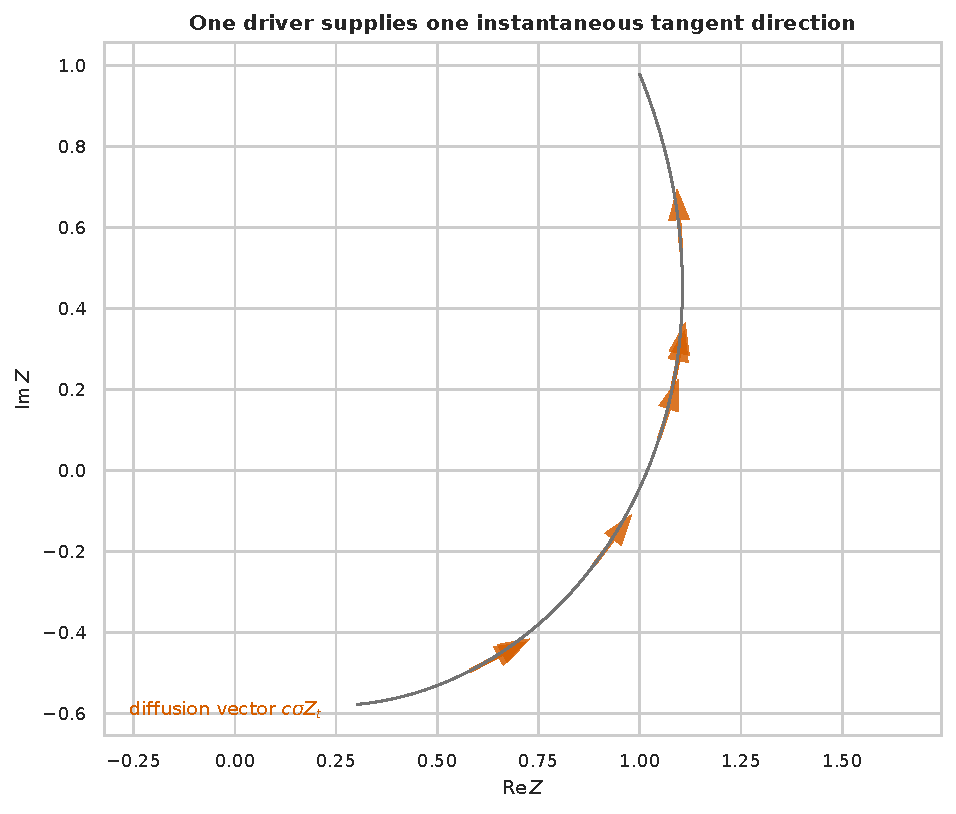
\includegraphics[width=0.7\linewidth,height=\textheight,keepaspectratio,alt={A logarithmic spiral has one red tangent arrow at each of several points. The arrows rotate along the curve but only one direction exists at any given point.}]{figures/vector/f06_local_noise_direction.pdf}

}

\caption{\label{fig-local-direction}Red arrows show the single diffusion
direction tangent to the supporting spiral at several states.}

\end{figure}%

The complex brackets follow immediately from the diffusion term:

\begin{equation}\protect\phantomsection\label{eq-complex-brackets}{
\boxed{
d[Z,Z]_t=c^2\sigma^2Z_t^2\,dt,\qquad
d[Z,\overline Z]_t=|c|^2\sigma^2|Z_t|^2\,dt.
}
}\end{equation}

\begin{figure}[H]

\centering{

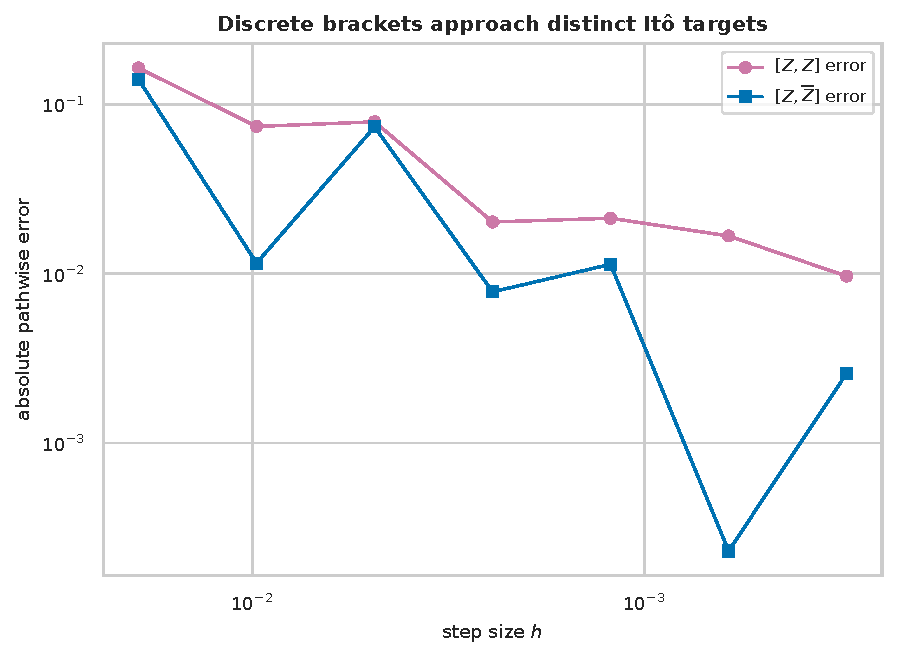
\includegraphics[width=0.7\linewidth,height=\textheight,keepaspectratio,alt={A log-log plot shows decreasing pathwise errors for the bilinear bracket Z Z and the Hermitian bracket Z conjugate Z across seven step sizes.}]{figures/vector/f18_complex_quadratic_variation.pdf}

}

\caption{\label{fig-complex-qv}Discrete bilinear and Hermitian bracket
sums approach their different Itô-integral targets as the grid is
refined.}

\end{figure}%

The pathwise convergence in Figure~\ref{fig-complex-qv} is irregular, as
expected for one sample path, but both finest-grid errors are
substantially below their coarsest-grid values.

Finally, \(Y_t=X_t-X_0\sim N(\mu t,\sigma^2t)\), so

\begin{equation}\protect\phantomsection\label{eq-radial-moments}{
\mathbb E[R_t^p]
=R_0^p\exp\!\left(
p\alpha\mu t+\tfrac12p^2\alpha^2\sigma^2t
\right)
}\end{equation}

and, for integers \(n\),

\begin{equation}\protect\phantomsection\label{eq-complex-moments}{
\mathbb E\!\left[\left(\frac{Z_t}{Z_0}\right)^n\right]
=\exp\!\left(
nc\mu t+\tfrac12n^2c^2\sigma^2t
\right).
}\end{equation}

\section{Noise dimension and covariance rank}\label{sec-rank}

The log-polar covariance density from Eq.~\ref{eq-linear-polar-sde} is

\begin{equation}\protect\phantomsection\label{eq-polar-covariance}{
K
=\sigma^2
\begin{pmatrix}
\alpha^2&\alpha\beta\\
\alpha\beta&\beta^2
\end{pmatrix}
=\sigma^2
\begin{pmatrix}\alpha\\\beta\end{pmatrix}
\begin{pmatrix}\alpha&\beta\end{pmatrix}.
}\end{equation}

Its eigenvalues are \(0\) and \(\sigma^2(\alpha^2+\beta^2)\). Both
coordinates fluctuate, but their local correlation has absolute value
one when \(\alpha\beta\ne0\).

\begin{theorem}[Rank-one theorem for scalar complex
images]\protect\hypertarget{thm-rank}{}\label{thm-rank}

Let

\[
dX_t=b_t\,dt+s_t\,dW_t
\]

be a scalar Itô process and let \(F=(F_1,F_2):\mathbb R\to\mathbb R^2\)
be \(C^2\). Then the instantaneous Cartesian covariance density of
\(F(X_t)\) is

\begin{equation}\protect\phantomsection\label{eq-general-rank-covariance}{
C_t=s_t^2F'(X_t)F'(X_t)^\mathsf T,
}\end{equation}

and therefore

\begin{equation}\protect\phantomsection\label{eq-rank-bound}{
\operatorname{rank}C_t\le1.
}\end{equation}

\end{theorem}

\textbf{Proof.} Componentwise Itô calculus gives

\[
dF_j(X_t)
=\left(b_tF_j'(X_t)+\tfrac12s_t^2F_j''(X_t)\right)dt
+s_tF_j'(X_t)dW_t.
\]

The two-dimensional diffusion matrix has the single column
\(s_tF'(X_t)\). Its covariance is the outer product in
Eq.~\ref{eq-general-rank-covariance}, whose rank is at most one.
\(\square\)

The same conclusion holds for any adapted two-dimensional Itô process
driven by one scalar Brownian motion:

\begin{equation}\protect\phantomsection\label{eq-stronger-rank}{
dY_t=q_t\,dt+v_t\,dW_t
\quad\Longrightarrow\quad
\frac{d[Y,Y]_t}{dt}=v_tv_t^\mathsf T.
}\end{equation}

Path dependence and state dependence can rotate \(v_t\), but cannot
create a second simultaneous noise direction.

For comparison only, isotropic planar Brownian motion

\begin{equation}\protect\phantomsection\label{eq-planar-control}{
d\widetilde Z_t=\sigma(dW_t^1+i\,dW_t^2)
}\end{equation}

has Cartesian covariance \(\sigma^2I_2\), of rank two. At a fixed
nonzero radius \(r\), its log-polar covariance is \((\sigma^2/r^2)I_2\).
The numerical control below uses \(r=1.30\), so its theoretical
log-polar eigenvalues are \(\sigma^2/r^2=0.4225/1.69=0.25\). This is a
distinct stochastic model with two independent Brownian drivers (Pitman
and Yor 2018).

\begin{figure}[H]

\centering{

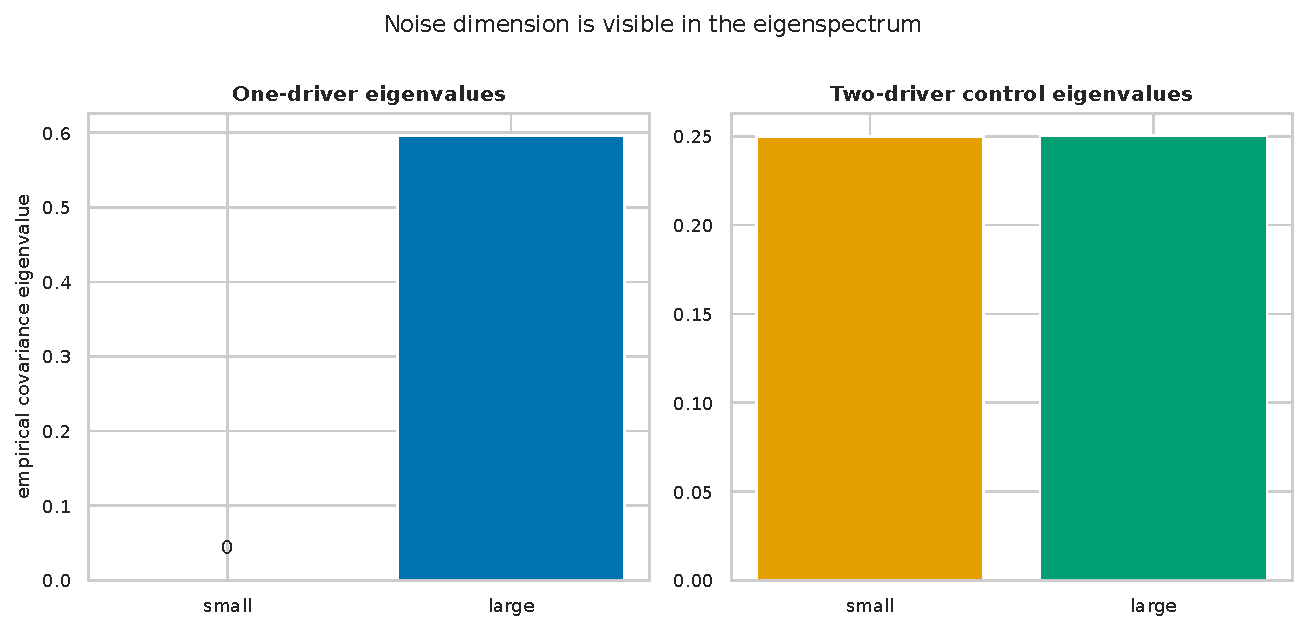
\includegraphics[width=0.78\linewidth,height=\textheight,keepaspectratio,alt={Two bar charts compare covariance eigenvalues. The one-driver chart has one zero and one positive bar. The two-driver chart has two nearly equal positive bars.}]{figures/vector/f07_covariance_eigenspectrum.pdf}

}

\caption{\label{fig-eigenspectrum}The empirical one-driver covariance
has one numerical-zero eigenvalue, while the two-driver control has two
positive eigenvalues.}

\end{figure}%

\begin{figure}[H]

\centering{

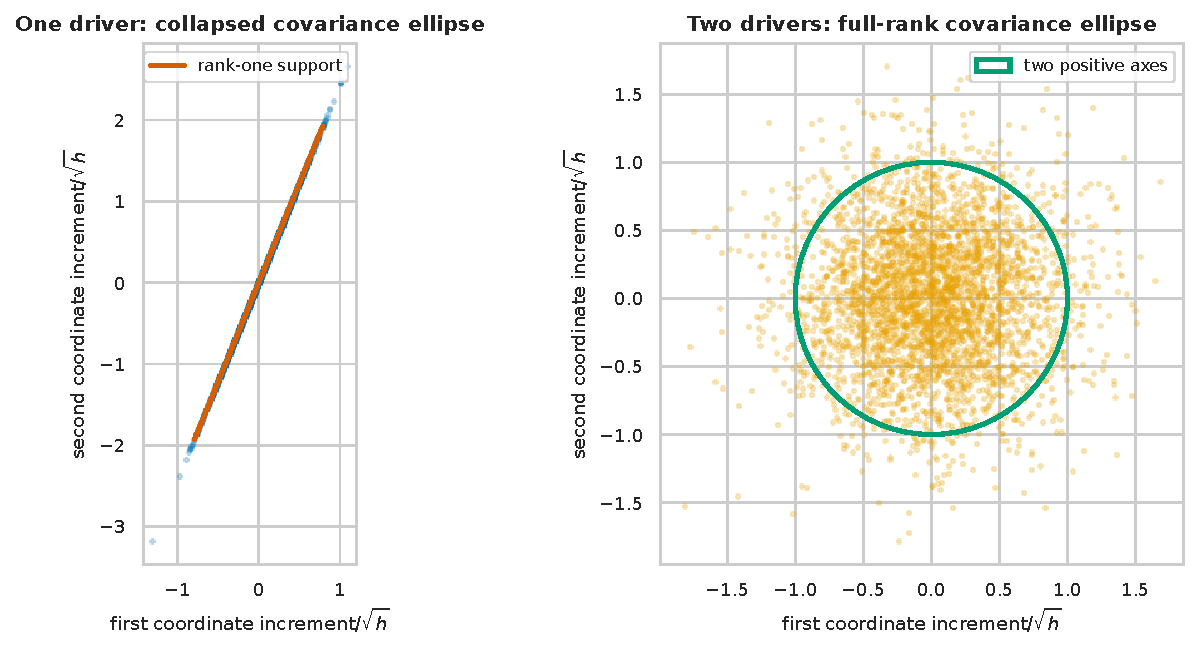
\includegraphics[width=0.92\linewidth,height=\textheight,keepaspectratio,alt={Two scatter plots show a thin line of one-driver increments and a circular cloud of two-driver increments, with the corresponding degenerate and full-rank covariance outlines.}]{figures/vector/f08_covariance_geometry.pdf}

}

\caption{\label{fig-covariance-geometry}Normalized one-driver increments
collapse to a line, while two-driver control increments occupy a
two-dimensional cloud.}

\end{figure}%

This distinction concerns the local covariance, not the long-time visual
support alone. A one-driver diffusion can trace a curved subset of the
plane, and a state-dependent one-driver diffusion can even have
two-dimensional support over time. At each instant, however, its
continuous martingale increment still lies in one direction.

\section{Scalar polar coordinates and zero crossings}\label{sec-zero}

A literal embedding of the signed scalar state is

\begin{equation}\protect\phantomsection\label{eq-real-axis}{
Z_t^{\mathrm{axis}}=X_t+i0.
}\end{equation}

Away from zero, \(R_t=|X_t|\) and \(\Theta_t=0\) for \(X_t>0\),
\(\Theta_t=\pi\) for \(X_t<0\). Let

\[
\tau_0=\inf\{t\ge0:X_t=0\}.
\]

On \(t<\tau_0\), scalar Itô calculus gives the localized identity

\begin{equation}\protect\phantomsection\label{eq-local-log}{
d\log|X_t|
=\left(\frac{\mu}{X_t}-\frac{\sigma^2}{2X_t^2}\right)dt
+\frac{\sigma}{X_t}\,dW_t.
}\end{equation}

This is exact on the stochastic interval before the zero, consistent
with the general need to stop logarithms at continuous zeros (Larsson
and Ruf 2019). It is not a global formula through sign changes.

The correct global formula for the radius is Tanaka's formula:

\begin{equation}\protect\phantomsection\label{eq-tanaka}{
\boxed{
|X_t|
=|X_0|
+\int_0^t\operatorname{sgn}(X_s)\,dX_s
+L_t^0(X).
}
}\end{equation}

Here \(L_t^0(X)\) is symmetric local time at zero (Mörters and Peres
2010; Biskup 2025). With constant volatility,

\begin{equation}\protect\phantomsection\label{eq-occupation-density}{
L_t^0(X)
=\lim_{\varepsilon\downarrow0}
\frac{1}{2\varepsilon}
\int_0^t\mathbf 1_{\{|X_s|<\varepsilon\}}\,d[X,X]_s
=\lim_{\varepsilon\downarrow0}
\frac{\sigma^2}{2\varepsilon}
\int_0^t\mathbf 1_{\{|X_s|<\varepsilon\}}\,ds
}\end{equation}

in the standard sense.

\begin{figure}[H]

\centering{

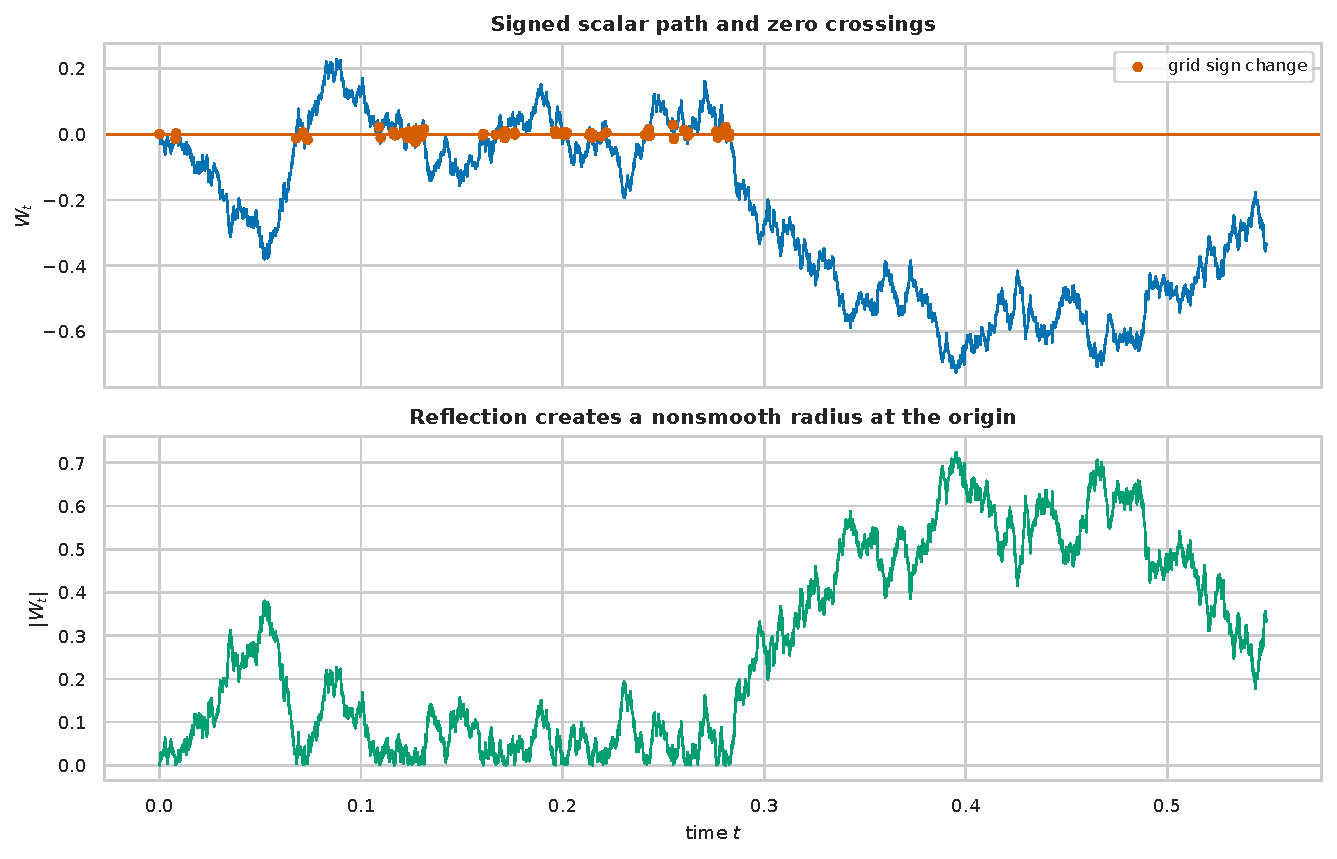
\includegraphics[width=0.88\linewidth,height=\textheight,keepaspectratio,alt={The top panel plots a Brownian path with marked sign changes at zero. The bottom panel plots its absolute value, showing reflection at the origin.}]{figures/vector/f13_zero_crossing_anatomy.pdf}

}

\caption{\label{fig-zero-crossings}A signed Brownian path crosses zero
while its absolute value reflects, creating the nonsmooth point that
invalidates a global ordinary logarithm.}

\end{figure}%

\begin{figure}[H]

\centering{

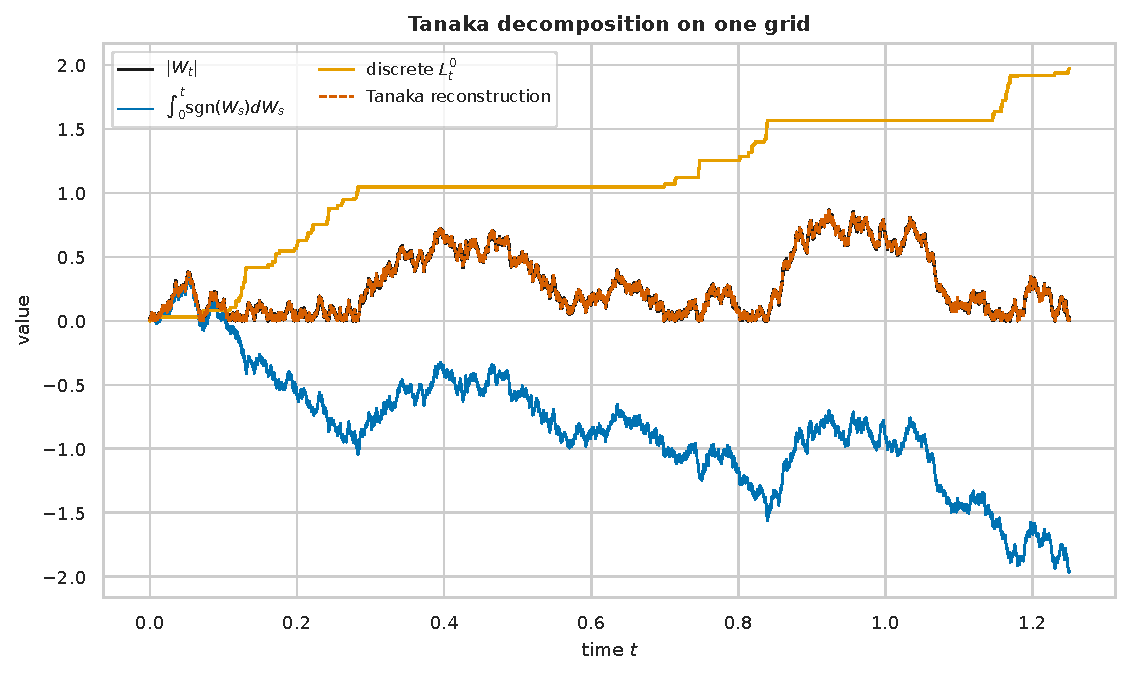
\includegraphics[width=0.88\linewidth,height=\textheight,keepaspectratio,alt={Four curves compare absolute Brownian motion, the stochastic sign integral, accumulated local time, and their Tanaka reconstruction. The reconstruction overlays the absolute path.}]{figures/vector/f14_tanaka_decomposition.pdf}

}

\caption{\label{fig-tanaka}The reflected path equals the stochastic sign
integral plus the accumulated discrete local-time residual.}

\end{figure}%

\begin{figure}[H]

\centering{

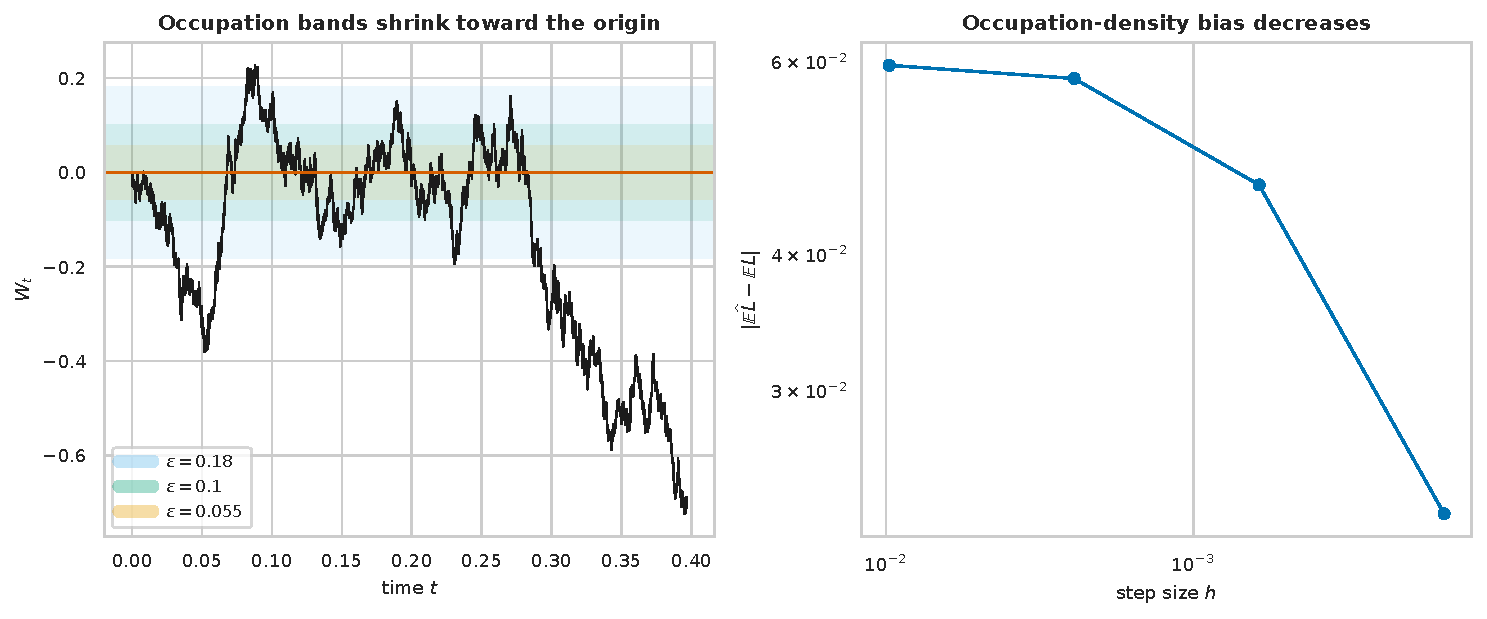
\includegraphics[width=0.92\linewidth,height=\textheight,keepaspectratio,alt={The left panel shows nested horizontal bands around zero on a Brownian path. The right panel shows decreasing absolute mean bias of an occupation-density local-time estimator.}]{figures/vector/f15_occupation_density.pdf}

}

\caption{\label{fig-occupation}Shrinking occupation bands concentrate
around zero, and the occupation-density bias decreases under joint grid
and bandwidth refinement.}

\end{figure}%

The logarithmic-spiral embedding avoids this singularity because
\(|Z_t|=R_0e^{\alpha(X_t-X_0)}>0\) for every finite \(X_t\). It should
not be confused with the literal polar coordinates of \(X_t+i0\); the
two representations answer different geometric questions.

\section{Numerical methods}\label{sec-methods}

The executable supplement is \texttt{notebooks/phase3\_discovery.ipynb}.
It was generated by \texttt{notebooks/build\_phase3\_discovery.py} and
executed from a clean kernel in the \texttt{phase3-paper} conda
environment.

The principal parameters were

\begin{equation}\protect\phantomsection\label{eq-numerical-parameters}{
\mu=0.20,\quad \sigma=0.65,\quad
\alpha=0.45,\quad\beta=1.10,\quad
X_0=-0.30,\quad R_0=1.20,\quad
\Theta_0=0.40,\quad T=1.25.
}\end{equation}

The master seed was \texttt{20260723}; independent experiments used
deterministic offsets from that seed.

The experiments were:

\begin{enumerate}
\def\labelenumi{\arabic{enumi}.}
\tightlist
\item
  exact Gaussian simulation of a 4096-step arithmetic Brownian path;
\item
  pathwise comparison of the direct map, cumulative exact products,
  inverse radius, and spiral constraint;
\item
  200,000 independent terminal draws for radial and complex moments;
\item
  250,000 local increments for rank-one and rank-two covariance
  estimates;
\item
  10,000 Brownian paths coupled across six Euler--Maruyama resolutions;
\item
  discrete bilinear and Hermitian bracket sums on seven nested grids;
\item
  a pathwise discrete Tanaka identity; and
\item
  6,000-path local-time estimates on four grids.
\end{enumerate}

For the exact discrete Tanaka check we used

\begin{equation}\protect\phantomsection\label{eq-discrete-tanaka-increment}{
\ell_n
=|W_{n+1}|-|W_n|-\operatorname{sgn}(W_n)\Delta W_n.
}\end{equation}

The sum of \(\ell_n\) closes the discrete identity algebraically. The
separate occupation estimator used

\begin{equation}\protect\phantomsection\label{eq-occupation-estimator}{
\widehat L_{T,\varepsilon,h}^0
=\frac1{2\varepsilon}
\sum_n\mathbf1_{\{|W_n|<\varepsilon\}}h,
\qquad \varepsilon=0.5h^{1/4}.
}\end{equation}

The analytic derivations are the proofs. Monte Carlo estimates test the
code, scale of uncertainty, and visual consequences.

\section{Numerical results}\label{sec-results}

\subsection{Pathwise identities}\label{pathwise-identities}

The maximum errors along the 4096-step path were:

\begin{longtable}[]{@{}lr@{}}
\caption{Pathwise exactness checks; the residuals are floating-point
roundoff.}\label{tbl-exactness}\tabularnewline
\toprule\noalign{}
Identity & Maximum absolute error \\
\midrule\noalign{}
\endfirsthead
\toprule\noalign{}
Identity & Maximum absolute error \\
\midrule\noalign{}
\endhead
\bottomrule\noalign{}
\endlastfoot
cumulative exact product versus direct \(Z_t\) &
\(6.273\times10^{-15}\) \\
\(X_t\) versus inverse-radius recovery & \(1.110\times10^{-15}\) \\
logarithmic-spiral constraint & \(5.274\times10^{-16}\) \\
\end{longtable}

The space-time view in Figure~\ref{fig-space-time} is intentionally
three-dimensional only to display temporal ordering. It must not be read
as evidence of a second planar noise direction.

\begin{figure}[H]

\centering{

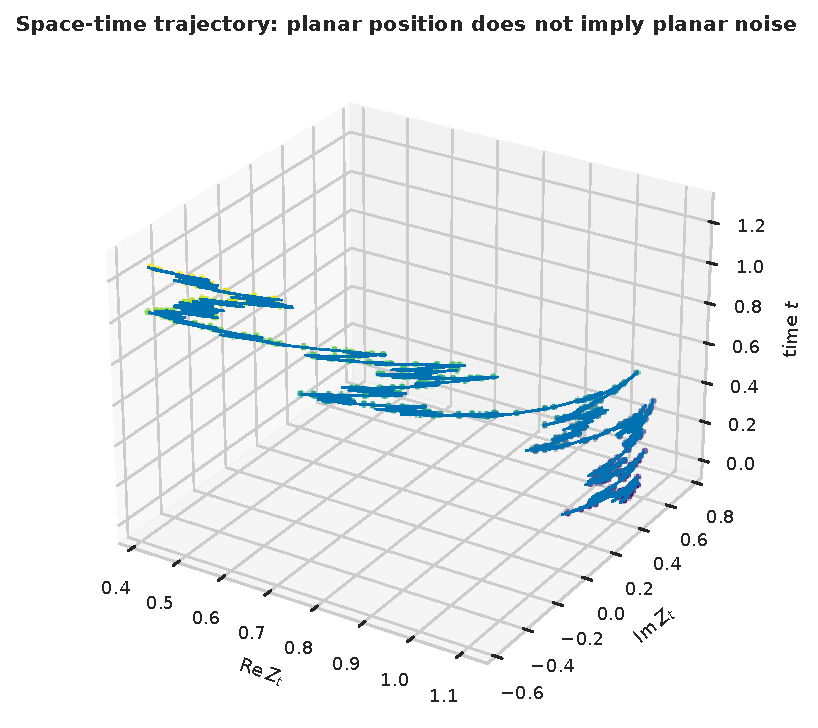
\includegraphics[width=0.75\linewidth,height=\textheight,keepaspectratio,alt={A three-dimensional curve plots real Z, imaginary Z, and time. It shows repeated motion along a spiral as time increases.}]{figures/vector/f04_space_time_trajectory.pdf}

}

\caption{\label{fig-space-time}Adding time as the third axis separates
repeated visits along the spiral without changing the one-driver
interpretation.}

\end{figure}%

\subsection{Distribution and moment
checks}\label{distribution-and-moment-checks}

The radial samples agree with the lognormal law implied by
Eq.~\ref{eq-radial-moments}.

\begin{figure}[H]

\centering{

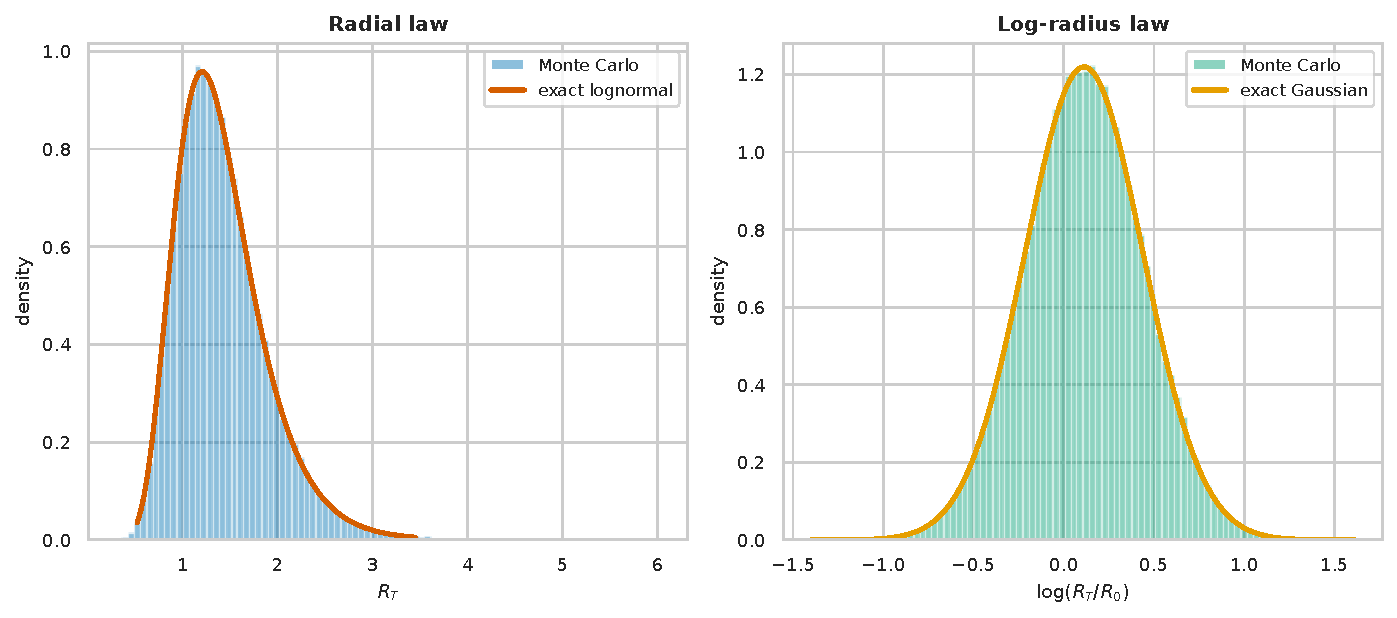
\includegraphics[width=0.88\linewidth,height=\textheight,keepaspectratio,alt={Two histograms show terminal radius with an exact lognormal curve and terminal log-radius with an exact Gaussian curve; the overlays closely agree.}]{figures/vector/f10_distribution_checks.pdf}

}

\caption{\label{fig-distributions}Monte Carlo histograms of radius and
log-radius overlay their exact lognormal and Gaussian densities.}

\end{figure}%

\begin{longtable}[]{@{}
  >{\raggedright\arraybackslash}p{(\linewidth - 10\tabcolsep) * \real{0.1667}}
  >{\raggedright\arraybackslash}p{(\linewidth - 10\tabcolsep) * \real{0.1667}}
  >{\raggedleft\arraybackslash}p{(\linewidth - 10\tabcolsep) * \real{0.1667}}
  >{\raggedleft\arraybackslash}p{(\linewidth - 10\tabcolsep) * \real{0.1667}}
  >{\raggedleft\arraybackslash}p{(\linewidth - 10\tabcolsep) * \real{0.1667}}
  >{\raggedleft\arraybackslash}p{(\linewidth - 10\tabcolsep) * \real{0.1667}}@{}}
\caption{Monte Carlo moment validation with 200,000 terminal
draws.}\label{tbl-moments}\tabularnewline
\toprule\noalign{}
\begin{minipage}[b]{\linewidth}\raggedright
Quantity
\end{minipage} & \begin{minipage}[b]{\linewidth}\raggedright
Component
\end{minipage} & \begin{minipage}[b]{\linewidth}\raggedleft
Estimate
\end{minipage} & \begin{minipage}[b]{\linewidth}\raggedleft
Exact
\end{minipage} & \begin{minipage}[b]{\linewidth}\raggedleft
Standard error
\end{minipage} & \begin{minipage}[b]{\linewidth}\raggedleft
\(z\)-score
\end{minipage} \\
\midrule\noalign{}
\endfirsthead
\toprule\noalign{}
\begin{minipage}[b]{\linewidth}\raggedright
Quantity
\end{minipage} & \begin{minipage}[b]{\linewidth}\raggedright
Component
\end{minipage} & \begin{minipage}[b]{\linewidth}\raggedleft
Estimate
\end{minipage} & \begin{minipage}[b]{\linewidth}\raggedleft
Exact
\end{minipage} & \begin{minipage}[b]{\linewidth}\raggedleft
Standard error
\end{minipage} & \begin{minipage}[b]{\linewidth}\raggedleft
\(z\)-score
\end{minipage} \\
\midrule\noalign{}
\endhead
\bottomrule\noalign{}
\endlastfoot
\(\mathbb E[R_T]\) & real & 1.415923 & 1.416649 & 0.001063 & -0.683 \\
\(\mathbb E[R_T^2]\) & real & 2.230873 & 2.233419 & 0.003636 & -0.700 \\
\(\mathbb E[Z_T/Z_0]\) & real & 0.737468 & 0.737199 & 0.001063 &
0.253 \\
\(\mathbb E[Z_T/Z_0]\) & imaginary & 0.437494 & 0.438321 & 0.001715 &
-0.482 \\
\(\mathbb E[(Z_T/Z_0)^2]\) & real & -0.009798 & -0.010754 & 0.003038 &
0.315 \\
\(\mathbb E[(Z_T/Z_0)^2]\) & imaginary & 0.431580 & 0.431934 & 0.002867
& -0.124 \\
\end{longtable}

\begin{figure}[H]

\centering{

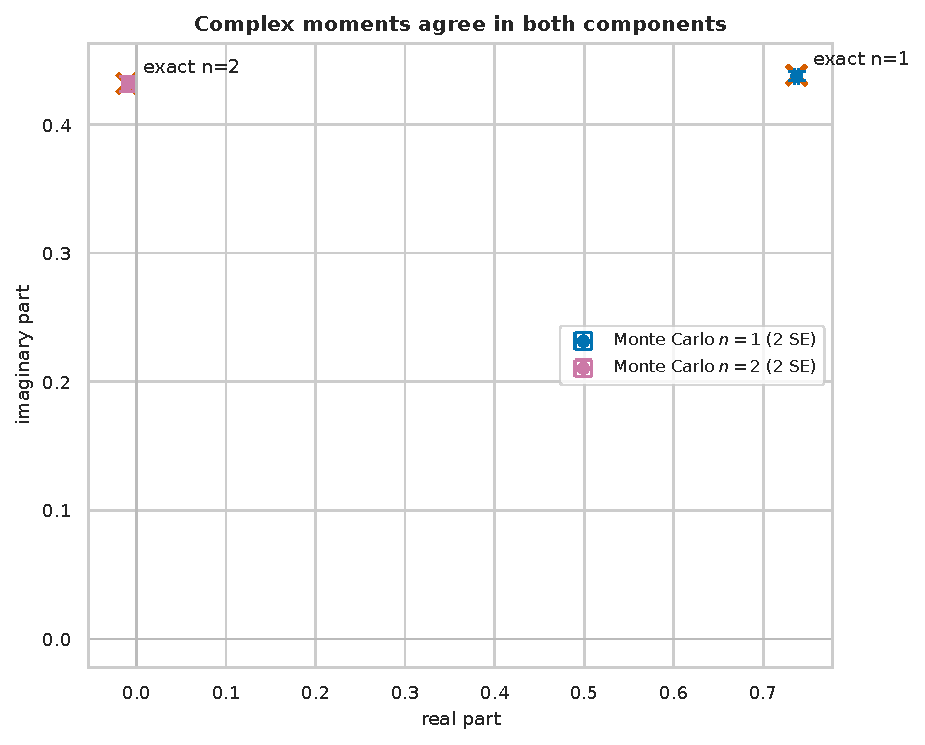
\includegraphics[width=0.68\linewidth,height=\textheight,keepaspectratio,alt={A complex-plane plot shows first and second empirical moments with horizontal and vertical two-standard-error bars beside exact cross markers.}]{figures/vector/f11_complex_moments.pdf}

}

\caption{\label{fig-complex-moments}Empirical complex moments with
two-standard-error bars coincide with their exact targets in the complex
plane.}

\end{figure}%

\subsection{Covariance rank}\label{covariance-rank}

\begin{longtable}[]{@{}
  >{\raggedright\arraybackslash}p{(\linewidth - 6\tabcolsep) * \real{0.2500}}
  >{\raggedleft\arraybackslash}p{(\linewidth - 6\tabcolsep) * \real{0.2500}}
  >{\raggedleft\arraybackslash}p{(\linewidth - 6\tabcolsep) * \real{0.2500}}
  >{\raggedleft\arraybackslash}p{(\linewidth - 6\tabcolsep) * \real{0.2500}}@{}}
\caption{Empirical log-polar covariance eigenspectra. The tiny negative
value is roundoff from a theoretically positive-semidefinite rank-one
matrix.}\label{tbl-covariance-results}\tabularnewline
\toprule\noalign{}
\begin{minipage}[b]{\linewidth}\raggedright
Model
\end{minipage} & \begin{minipage}[b]{\linewidth}\raggedleft
Small eigenvalue
\end{minipage} & \begin{minipage}[b]{\linewidth}\raggedleft
Large eigenvalue
\end{minipage} & \begin{minipage}[b]{\linewidth}\raggedleft
Relative matrix error
\end{minipage} \\
\midrule\noalign{}
\endfirsthead
\toprule\noalign{}
\begin{minipage}[b]{\linewidth}\raggedright
Model
\end{minipage} & \begin{minipage}[b]{\linewidth}\raggedleft
Small eigenvalue
\end{minipage} & \begin{minipage}[b]{\linewidth}\raggedleft
Large eigenvalue
\end{minipage} & \begin{minipage}[b]{\linewidth}\raggedleft
Relative matrix error
\end{minipage} \\
\midrule\noalign{}
\endhead
\bottomrule\noalign{}
\endlastfoot
one-driver log-polar embedding & \(-1.39\times10^{-16}\) & 0.595978 &
0.00135 \\
two-driver log-polar control (\(r=1.30\)) & 0.249766 & 0.250352 &
0.00120 \\
\end{longtable}

These values numerically expose the exact rank distinction already
proved in Theorem~\ref{thm-rank}. The experiment is a check of
implementation, not an independent proof.

\subsection{Strong convergence}\label{strong-convergence}

\begin{longtable}[]{@{}rrrr@{}}
\caption{Coupled Euler--Maruyama strong
errors.}\label{tbl-convergence}\tabularnewline
\toprule\noalign{}
Steps \(N\) & \(h\) & Mean terminal error & Standard error \\
\midrule\noalign{}
\endfirsthead
\toprule\noalign{}
Steps \(N\) & \(h\) & Mean terminal error & Standard error \\
\midrule\noalign{}
\endhead
\bottomrule\noalign{}
\endlastfoot
16 & 0.078125 & 0.150392 & 0.001469 \\
32 & 0.0390625 & 0.106417 & 0.000972 \\
64 & 0.0195313 & 0.075794 & 0.000690 \\
128 & 0.00976563 & 0.052824 & 0.000455 \\
256 & 0.00488281 & 0.037456 & 0.000311 \\
512 & 0.00244141 & 0.026537 & 0.000229 \\
\end{longtable}

The fitted log-log slope was \(0.5015\), consistent with strong order
\(1/2\) (Higham 2001).

\begin{figure}[H]

\centering{

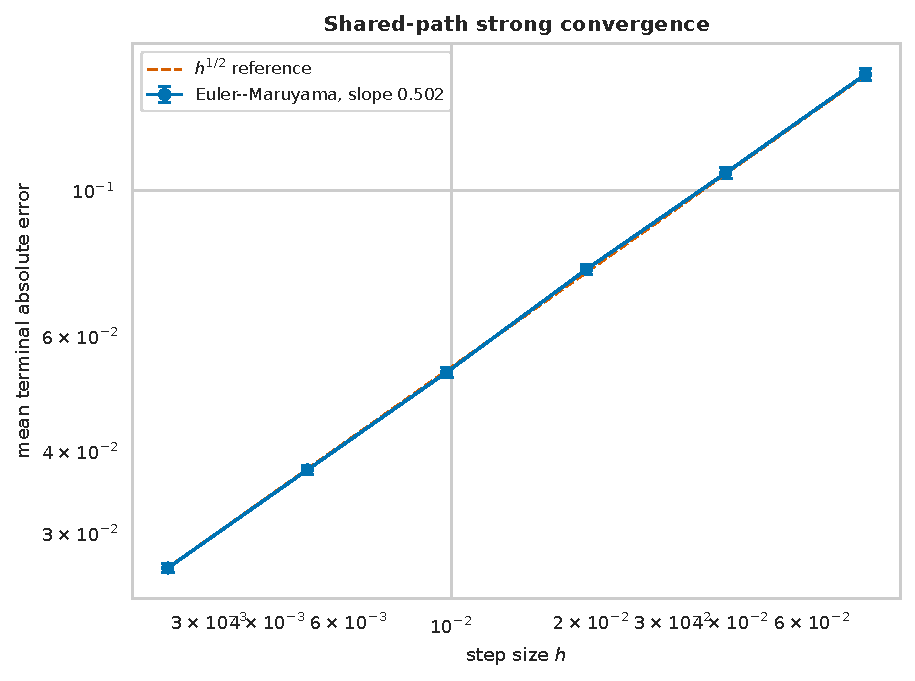
\includegraphics[width=0.7\linewidth,height=\textheight,keepaspectratio,alt={A log-log graph plots mean Euler-\/-Maruyama terminal error with uncertainty bars and a dashed h to the one-half reference line. The fitted slope is about 0.502.}]{figures/vector/f12_strong_convergence.pdf}

}

\caption{\label{fig-strong-convergence}The shared-path Euler--Maruyama
errors follow the half-order reference line.}

\end{figure}%

\subsection{Local time}\label{local-time}

For standard Brownian motion over \(T=1.25\),

\[
\mathbb E[L_T^0]=\sqrt{\frac{2T}{\pi}}=0.892062.
\]

\begin{longtable}[]{@{}
  >{\raggedleft\arraybackslash}p{(\linewidth - 10\tabcolsep) * \real{0.1667}}
  >{\raggedleft\arraybackslash}p{(\linewidth - 10\tabcolsep) * \real{0.1667}}
  >{\raggedleft\arraybackslash}p{(\linewidth - 10\tabcolsep) * \real{0.1667}}
  >{\raggedleft\arraybackslash}p{(\linewidth - 10\tabcolsep) * \real{0.1667}}
  >{\raggedleft\arraybackslash}p{(\linewidth - 10\tabcolsep) * \real{0.1667}}
  >{\raggedleft\arraybackslash}p{(\linewidth - 10\tabcolsep) * \real{0.1667}}@{}}
\caption{Discrete Tanaka and occupation-density results over 6,000
paths.}\label{tbl-local-time}\tabularnewline
\toprule\noalign{}
\begin{minipage}[b]{\linewidth}\raggedleft
Steps \(N\)
\end{minipage} & \begin{minipage}[b]{\linewidth}\raggedleft
\(\varepsilon\)
\end{minipage} & \begin{minipage}[b]{\linewidth}\raggedleft
Discrete mean
\end{minipage} & \begin{minipage}[b]{\linewidth}\raggedleft
Occupation mean
\end{minipage} & \begin{minipage}[b]{\linewidth}\raggedleft
Occupation absolute error
\end{minipage} & \begin{minipage}[b]{\linewidth}\raggedleft
Identity max error
\end{minipage} \\
\midrule\noalign{}
\endfirsthead
\toprule\noalign{}
\begin{minipage}[b]{\linewidth}\raggedleft
Steps \(N\)
\end{minipage} & \begin{minipage}[b]{\linewidth}\raggedleft
\(\varepsilon\)
\end{minipage} & \begin{minipage}[b]{\linewidth}\raggedleft
Discrete mean
\end{minipage} & \begin{minipage}[b]{\linewidth}\raggedleft
Occupation mean
\end{minipage} & \begin{minipage}[b]{\linewidth}\raggedleft
Occupation absolute error
\end{minipage} & \begin{minipage}[b]{\linewidth}\raggedleft
Identity max error
\end{minipage} \\
\midrule\noalign{}
\endhead
\bottomrule\noalign{}
\endlastfoot
128 & 0.157179 & 0.895332 & 0.832549 & 0.059513 &
\(2.82\times10^{-15}\) \\
512 & 0.111142 & 0.882717 & 0.834180 & 0.057882 &
\(7.11\times10^{-15}\) \\
2048 & 0.078590 & 0.884203 & 0.845796 & 0.046266 &
\(1.07\times10^{-14}\) \\
8192 & 0.055571 & 0.893896 & 0.868905 & 0.023157 &
\(2.00\times10^{-14}\) \\
\end{longtable}

The discrete identity closes to roundoff on every grid. The occupation
estimator has visible finite-bandwidth bias, which decreases but
converges more slowly. This is why exact grid hits are not used as a
local-time estimator.

\section{Discussion}\label{sec-discussion}

The construction resolves the apparent tension between a stochastic
radius and a scalar Brownian driver. A random radius does not imply
two-dimensional noise. In Eq.~\ref{eq-polar-coordinates}, both
log-radius and angle are random because both depend on \(X_t\). They are
nevertheless perfectly locally coupled, as Eq.~\ref{eq-spiral-relation}
and Eq.~\ref{eq-polar-covariance} show.

The embedding preserves more than a visual trace. For \(\alpha\ne0\),
Eq.~\ref{eq-inverse-radius} reconstructs the scalar state at every time,
so the complex and scalar processes generate the same information. Yet
it preserves less than a full planar model: no deterministic or adapted
transformation driven by one scalar Brownian motion can match a
positive-definite instantaneous two-dimensional covariance.

This distinction clarifies the roles of \(i\) and quadratic variation:

\begin{itemize}
\tightlist
\item
  multiplication by \(i\) rotates a complex vector by \(90^\circ\);
\item
  the imaginary part of \(c\) converts a scalar displacement into phase;
\item
  \(i^2=-1\) is exact complex algebra;
\item
  \([W,W]_t=t\) is a pathwise limit of squared increments; and
\item
  the Itô drift correction in Eq.~\ref{eq-complex-sde} comes from the
  second derivative and quadratic variation, not from treating \(dW\) as
  an ordinary square root of \(dt\).
\end{itemize}

\begin{figure}[H]

\centering{

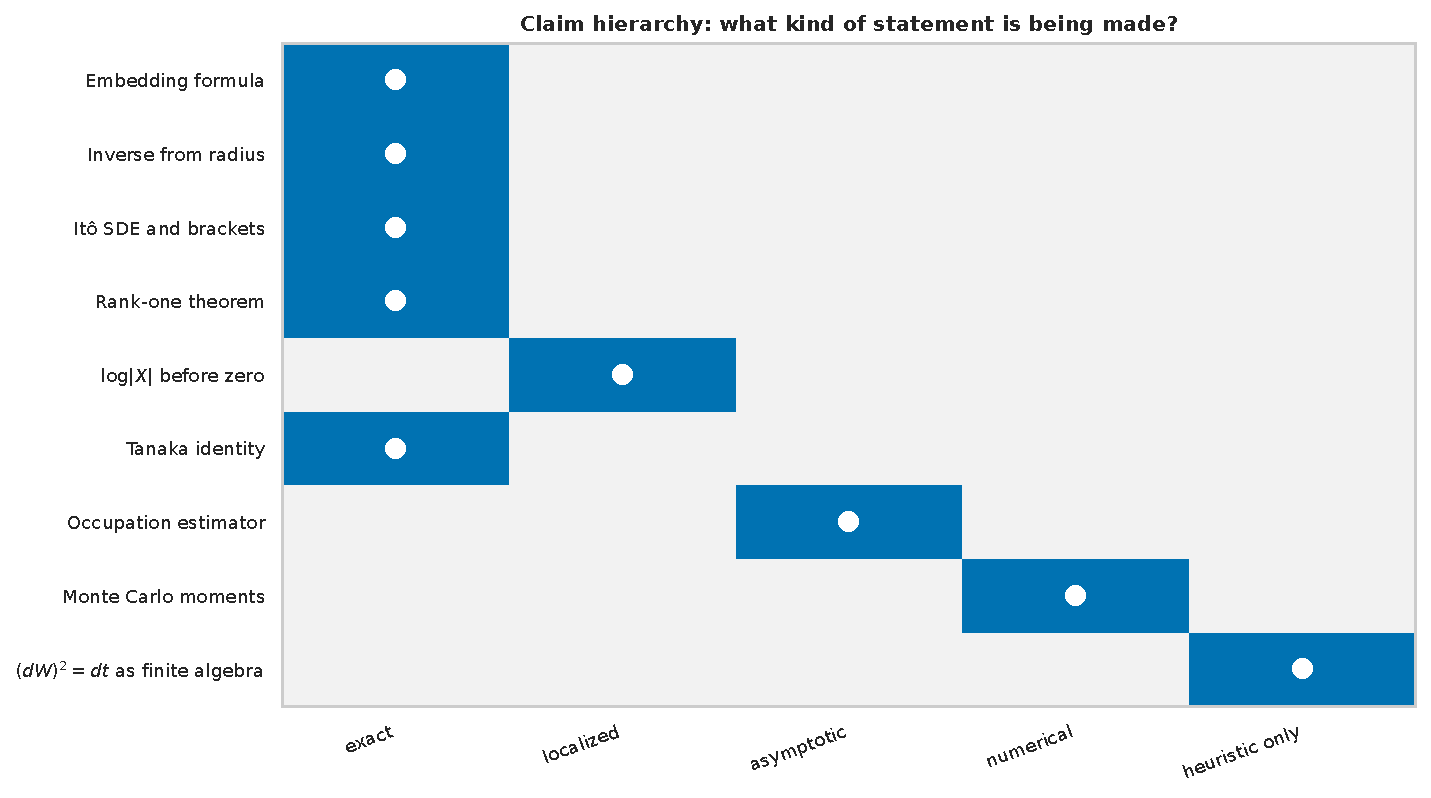
\includegraphics[width=0.88\linewidth,height=\textheight,keepaspectratio,alt={A matrix marks the embedding, inverse, Itô SDE, rank theorem, and Tanaka identity as exact; log absolute X as localized; occupation estimation as asymptotic; Monte Carlo as numerical; and finite differential algebra as heuristic only.}]{figures/vector/f17_claim_hierarchy.pdf}

}

\caption{\label{fig-claim-hierarchy}The notebook classifies each major
statement as exact, localized, asymptotic, numerical, or heuristic.}

\end{figure}%

Figure~\ref{fig-claim-hierarchy} is a compact guard against
overinterpretation. In particular, the finite-increment statement
\((\Delta W)^2=\Delta t\) is false pathwise. Only aggregated squared
increments converge to elapsed time.

\section{Limitations}\label{sec-limitations}

The construction has clear boundaries.

\begin{enumerate}
\def\labelenumi{\arabic{enumi}.}
\tightlist
\item
  It is a deterministic embedding of a scalar process, not a universal
  model of planar stochastic motion.
\item
  When \(\alpha=0\), radius no longer provides pointwise recovery. A
  continuously lifted phase can preserve the scalar path, but the
  wrapped complex state need not be injective.
\item
  The literal real-axis polar form is singular at zero; localization and
  Tanaka local time are structural necessities, not numerical nuisances.
\item
  The covariance theorem concerns instantaneous continuous-martingale
  rank. It does not assert that every one-driver process has
  one-dimensional long-time support.
\item
  The occupation-density estimator converges slowly because grid and
  bandwidth limits interact.
\item
  Monte Carlo results validate implementation and scale; they do not
  prove the analytic identities.
\item
  No claim of historical novelty is made for the logarithmic-spiral map
  or the rank-one outer-product argument.
\end{enumerate}

\section{Conclusion}\label{sec-conclusion}

A scalar arithmetic Brownian motion has the faithful complex form

\[
Z_t=Z_0e^{(\alpha+i\beta)(X_t-X_0)},\qquad \alpha\ne0,
\]

with both stochastic radius and stochastic angle. Its induced Itô
dynamics are

\[
\frac{dZ_t}{Z_t}
=\left[
(\alpha+i\beta)\mu
+\frac12(\alpha+i\beta)^2\sigma^2
\right]dt
+(\alpha+i\beta)\sigma\,dW_t,
\]

and its exact random-walk step is

\[
Z_{n+1}
=Z_n\exp\!\left[
(\alpha+i\beta)
(\mu\Delta t+\sigma\Delta W_n)
\right].
\]

The radius reconstructs \(X_t\); the angle supplies a geometric
rotation; and the shared Brownian increment forces rank-one local
covariance. A genuine planar Brownian motion remains a different,
rank-two, two-driver model. At scalar zero crossings, the ordinary polar
logarithm must give way to localization and Tanaka local time.

The bridge between complex numbers and Itô calculus is therefore precise
but limited: complex exponentials organize stochastic scale and
rotation, while quadratic variation---not the algebraic identity
\(i^2=-1\)---produces the Itô correction.

\section{Appendix A. Expanded Itô algebra}\label{sec-appendix-ito}

Starting from Eq.~\ref{eq-polar-reconstruction} and
Eq.~\ref{eq-linear-polar-sde},

\[
\begin{aligned}
\frac{dZ}{Z}
&=\alpha\mu\,dt+\alpha\sigma\,dW
  +i\beta\mu\,dt+i\beta\sigma\,dW\\
&\quad+\frac12(\alpha^2-\beta^2)\sigma^2dt
  +i\alpha\beta\sigma^2dt\\
&=\left[
(\alpha+i\beta)\mu
+\frac12(\alpha^2-\beta^2+2i\alpha\beta)\sigma^2
\right]dt\\
&\quad+(\alpha+i\beta)\sigma\,dW\\
&=\left(c\mu+\frac12c^2\sigma^2\right)dt+c\sigma\,dW.
\end{aligned}
\]

The symbolic notebook independently simplifies the difference between
the direct and polar drifts to zero.

\section{Appendix B. Exact moment
derivation}\label{sec-appendix-moments}

For any complex \(q\), the entire Gaussian moment-generating function
gives

\[
\mathbb E[e^{qY_t}]
=\exp\!\left(q\mu t+\tfrac12q^2\sigma^2t\right),
\qquad Y_t=X_t-X_0.
\]

Taking \(q=p\alpha\) and multiplying by \(R_0^p\) gives
Eq.~\ref{eq-radial-moments}. Taking \(q=nc\) gives
Eq.~\ref{eq-complex-moments}. No complex branch choice appears because
the random variable is defined by the entire exponential function, not
by applying a logarithm to sampled \(Z_t\).

\section{Appendix C. Reproducibility
manifest}\label{sec-reproducibility}

The preserved execution used:

\begin{longtable}[]{@{}ll@{}}
\caption{Software used for the executed notebook and
manuscript.}\label{tbl-software}\tabularnewline
\toprule\noalign{}
Component & Version \\
\midrule\noalign{}
\endfirsthead
\toprule\noalign{}
Component & Version \\
\midrule\noalign{}
\endhead
\bottomrule\noalign{}
\endlastfoot
Python & 3.12.13 \\
NumPy & 2.5.1 \\
SciPy & 1.18.0 \\
pandas & 3.0.3 \\
Matplotlib & 3.11.1 \\
Seaborn & 0.13.2 \\
SymPy & 1.14.0 \\
nbformat & 5.10.4 \\
Quarto & 1.9.38 \\
TinyTeX & 2026 \\
\end{longtable}

From the repository root, regenerate and execute the notebook with:

\begin{Shaded}
\begin{Highlighting}[]
\ExtensionTok{conda}\NormalTok{ run }\AttributeTok{{-}n}\NormalTok{ phase3{-}paper python }\DataTypeTok{\textbackslash{}}
\NormalTok{  paper/notebooks/build\_phase3\_discovery.py}

\ExtensionTok{conda}\NormalTok{ run }\AttributeTok{{-}n}\NormalTok{ phase3{-}paper jupyter nbconvert }\DataTypeTok{\textbackslash{}}
  \AttributeTok{{-}{-}to}\NormalTok{ notebook }\AttributeTok{{-}{-}execute} \AttributeTok{{-}{-}inplace} \DataTypeTok{\textbackslash{}}
  \AttributeTok{{-}{-}ExecutePreprocessor.timeout}\OperatorTok{=}\NormalTok{900 }\DataTypeTok{\textbackslash{}}
\NormalTok{  paper/notebooks/phase3\_discovery.ipynb}
\end{Highlighting}
\end{Shaded}

Then render the paper:

\begin{Shaded}
\begin{Highlighting}[]
\ExtensionTok{quarto}\NormalTok{ render paper }\AttributeTok{{-}{-}to}\NormalTok{ pdf}
\end{Highlighting}
\end{Shaded}

The notebook writes all figure sources to \texttt{paper/figures/}, all
numerical tables to \texttt{paper/tables/}, and a machine-readable
summary to \texttt{paper/tables/numerical\_summary.json}.

\protect\phantomsection\label{refs}
\begin{CSLReferences}{1}{1}
\bibitem[\citeproctext]{ref-biskup2025localtime}
Biskup, Marek. 2025. \emph{Brownian Local Time}. MATH 275D Notes,
Chapter 29, University of California, Los Angeles.
\url{https://www.math.ucla.edu/~biskup/275d.1.25f/PDFs/ch29.pdf}.

\bibitem[\citeproctext]{ref-goodman2007ito}
Goodman, Jonathan. 2007. \emph{Stochastic Calculus Notes: Lecture 8}.
Courant Institute of Mathematical Sciences, New York University.
\url{https://math.nyu.edu/~goodman/teaching/StochCalc2007/notes/l8.pdf}.

\bibitem[\citeproctext]{ref-higham2001}
Higham, Desmond J. 2001. {``An Algorithmic Introduction to Numerical
Simulation of Stochastic Differential Equations.''} \emph{SIAM Review}
43 (3): 525--46. \url{https://doi.org/10.1137/S0036144500378302}.

\bibitem[\citeproctext]{ref-larssonruf2019}
Larsson, Martin, and Johannes Ruf. 2019. {``Stochastic Exponentials and
Logarithms on Stochastic Intervals---a Survey.''} \emph{Journal of
Mathematical Analysis and Applications} 476 (1): 2--12.
\url{https://doi.org/10.1016/j.jmaa.2018.11.040}.

\bibitem[\citeproctext]{ref-mortersperes2010}
Mörters, Peter, and Yuval Peres. 2010. \emph{Brownian Motion}. Cambridge
Series in Statistical and Probabilistic Mathematics 30. Cambridge
University Press. \url{https://doi.org/10.1017/CBO9780511750489}.

\bibitem[\citeproctext]{ref-pitmanyor1986}
Pitman, Jim, and Marc Yor. 1986. {``Asymptotic Laws of Planar Brownian
Motion.''} \emph{The Annals of Probability} 14 (3): 733--79.
\url{https://www.jstor.org/stable/2244132}.

\bibitem[\citeproctext]{ref-pitmanyor2018guide}
Pitman, Jim, and Marc Yor. 2018. \emph{A Guide to Brownian Motion and
Related Stochastic Processes}. \url{https://arxiv.org/abs/1802.09679}.

\end{CSLReferences}




\end{document}
